
%% LyX 2.2.1 created this file.  For more info, see http://www.lyx.org/.
%% Do not edit unless you really know what you are doing.
\documentclass[12pt, usenames, dvipsnames]{beamer}\usepackage[]{graphicx}\usepackage[]{color}
%% maxwidth is the original width if it is less than linewidth
%% otherwise use linewidth (to make sure the graphics do not exceed the margin)
\makeatletter
\def\maxwidth{ %
  \ifdim\Gin@nat@width>\linewidth
    \linewidth
  \else
    \Gin@nat@width
  \fi
}
\makeatother

\definecolor{fgcolor}{rgb}{0.345, 0.345, 0.345}
\newcommand{\hlnum}[1]{\textcolor[rgb]{0.686,0.059,0.569}{#1}}%
\newcommand{\hlstr}[1]{\textcolor[rgb]{0.192,0.494,0.8}{#1}}%
\newcommand{\hlcom}[1]{\textcolor[rgb]{0.678,0.584,0.686}{\textit{#1}}}%
\newcommand{\hlopt}[1]{\textcolor[rgb]{0,0,0}{#1}}%
\newcommand{\hlstd}[1]{\textcolor[rgb]{0.345,0.345,0.345}{#1}}%
\newcommand{\hlkwa}[1]{\textcolor[rgb]{0.161,0.373,0.58}{\textbf{#1}}}%
\newcommand{\hlkwb}[1]{\textcolor[rgb]{0.69,0.353,0.396}{#1}}%
\newcommand{\hlkwc}[1]{\textcolor[rgb]{0.333,0.667,0.333}{#1}}%
\newcommand{\hlkwd}[1]{\textcolor[rgb]{0.737,0.353,0.396}{\textbf{#1}}}%
\let\hlipl\hlkwb

\usepackage{framed}
\makeatletter
\newenvironment{kframe}{%
 \def\at@end@of@kframe{}%
 \ifinner\ifhmode%
  \def\at@end@of@kframe{\end{minipage}}%
  \begin{minipage}{\columnwidth}%
 \fi\fi%
 \def\FrameCommand##1{\hskip\@totalleftmargin \hskip-\fboxsep
 \colorbox{shadecolor}{##1}\hskip-\fboxsep
     % There is no \\@totalrightmargin, so:
     \hskip-\linewidth \hskip-\@totalleftmargin \hskip\columnwidth}%
 \MakeFramed {\advance\hsize-\width
   \@totalleftmargin\z@ \linewidth\hsize
   \@setminipage}}%
 {\par\unskip\endMakeFramed%
 \at@end@of@kframe}
\makeatother

\definecolor{shadecolor}{rgb}{.97, .97, .97}
\definecolor{messagecolor}{rgb}{0, 0, 0}
\definecolor{warningcolor}{rgb}{1, 0, 1}
\definecolor{errorcolor}{rgb}{1, 0, 0}
\newenvironment{knitrout}{}{} % an empty environment to be redefined in TeX

\usepackage{alltt}
\usepackage[T1]{fontenc}
\usepackage[utf8]{inputenc}
\setcounter{secnumdepth}{3}
\setcounter{tocdepth}{3}
\usepackage{url}
\ifx\hypersetup\undefined
  \AtBeginDocument{%
    \hypersetup{unicode=true,pdfusetitle,
 bookmarks=true,bookmarksnumbered=false,bookmarksopen=false,
 breaklinks=false,pdfborder={0 0 0},pdfborderstyle={},backref=false,colorlinks=false}
  }
\else
  \hypersetup{unicode=true,pdfusetitle,
 bookmarks=true,bookmarksnumbered=false,bookmarksopen=false,
 breaklinks=false,pdfborder={0 0 0},pdfborderstyle={},backref=false,colorlinks=false}
\fi
\usepackage{breakurl}
\usepackage{xspace}
\usepackage{array}
\usepackage{xcolor}
\newcommand{\while}{{\tt while}\xspace}
\makeatletter

\definecolor{dimgray}{rgb}{0.41, 0.41, 0.41}
\definecolor{blue(ncs)}{rgb}{0.0, 0.53, 0.74}
% R arguments/parameters
\newcommand{\rp}[1]{\textcolor{Green}{\tt #1}}
% R functions
\newcommand{\rf}[1]{\textcolor{BrickRed}{\tt #1}}
% R characters
\newcommand{\rc}[1]{\textcolor{blue(ncs)}{\tt #1}}
% R values and reserved words
\newcommand{\rv}[1]{\textcolor{RedViolet}{\tt #1}}
% R objects
\newcommand{\ro}[1]{\textcolor{dimgray}{\tt #1}} 
% R text/commans
\newcommand{\rt}[1]{\textcolor{dimgray}{\tt #1}}

\usepackage{xspace}

\newcommand{\ggplot}{\rf{ggplot()}\xspace}
\newcommand{\ggpp}{\rt{ggplot2}\xspace}

%%%% https://www.overleaf.com/learn/latex/LaTeX_Graphics_using_TikZ:_A_Tutorial_for_Beginners_(Part_3)%E2%80%94Creating_Flowcharts
\usepackage{tikz}
\usetikzlibrary{shapes.geometric, arrows}

\tikzstyle{startstop} = [rectangle, rounded corners, minimum width=2cm, minimum height=0.75cm,text centered, draw=black, fill=red!30]

\tikzstyle{io} = [rectangle, minimum width=2cm, minimum height=1cm, text centered, draw=black, fill=blue!30]

\tikzstyle{process} = [rectangle, minimum width=2cm, minimum height=0.75cm, text centered, draw=black, fill=orange!30]
\tikzstyle{decision} = [diamond, minimum width=2cm, minimum height=1cm, text centered, draw=black, fill=green!30]

\tikzstyle{arrow} = [thick,->,>=stealth]
%%%%%%%%%%%%%%

\usetikzlibrary{shapes.geometric, arrows,chains}
\tikzset{
%  startstop/.style={
%    rectangle, 
%    rounded corners,
%    minimum width=3cm, 
%    minimum height=1cm,
%    align=center, 
%    draw=black, 
%    fill=red!30
%    },
%  process/.style={
%    rectangle, 
%    minimum width=3cm, 
%    minimum height=1cm, 
%    align=center, 
%    draw=black, 
%    fill=blue!30
%    },
  decision/.style={
    diamond, 
    minimum width=3cm, 
    minimum height=1cm, align=center, 
    draw=black, 
    fill=green!30
    },
  arrow/.style={thick,->,>=stealth},
  dec/.style={
    ellipse, 
    align=center, 
    draw=black, 
    fill=green!30
    },
}



%%%%%%%%%%%%%%%%%%%%%%%%%%%%%% LyX specific LaTeX commands.
\providecommand{\LyX}{\texorpdfstring%
  {L\kern-.1667em\lower.25em\hbox{Y}\kern-.125emX\@}
  {LyX}}

%%%%%%%%%%%%%%%%%%%%%%%%%%%%%% Textclass specific LaTeX commands.
 % this default might be overridden by plain title style
 \newcommand\makebeamertitle{\frame{\maketitle}}%
 % (ERT) argument for the TOC
 \AtBeginDocument{%
   \let\origtableofcontents=\tableofcontents
   \def\tableofcontents{\@ifnextchar[{\origtableofcontents}{\gobbletableofcontents}}
   \def\gobbletableofcontents#1{\origtableofcontents}
 }
 
 \renewenvironment{knitrout}{\setlength{\topsep}{0mm}}{} 

%%%%%%%%%%%%%%%%%%%%%%%%%%%%%% User specified LaTeX commands.
\usetheme{default}

\makeatother

 \usepackage[utf8]{inputenc}
\usepackage[T1]{fontenc}
\usepackage[english]{babel}

%\usepackage{verbatim}

\usepackage[export]{adjustbox}

\usepackage{
    amsmath,
    amsfonts,
    etex,
    fancyvrb,
    graphicx,
    multicol,
    pifont,
    setspace,
    soul,
    spverbatim,
    textcomp,
    xcolor,
    xspace
}

\usepackage{tikz}
\usetikzlibrary{shadows}

%%%SETUP%%%
\hypersetup{
     colorlinks = true,
     linkcolor = blue,
     anchorcolor = blue,
     citecolor = blue,
     filecolor = blue,
     urlcolor = blue
     }
     
%%%THEOREMS%%%
\theoremstyle{example}
\newtheorem*{exercise}{Exercise}
\newtheorem*{question}{Question}
\newtheorem*{answer}{\emph{Answer}}
\newtheorem*{notation}{Notation}

%%%TWEAKS%%%
\setlength\arraycolsep{4pt}
\addtolength\fboxsep{10pt}
\setstretch{1.4}
\setbeamersize{description width=3em}
\setbeamersize{text margin left=.5cm,text margin right=.5cm} 
\renewcommand{\emph}{\alert}
\renewcommand{\arraystretch}{1.2}
\renewcommand{\tabcolsep}{4pt}
\setbeamercolor{alerted text}{fg=magenta}


\graphicspath{{img/}}

%for straight quotes in verbatim:
\usepackage{upquote,textcomp}

%turn off navigation symbols
\beamertemplatenavigationsymbolsempty
\setbeamertemplate{footline}[frame number]

%title page

\author
  [Dr.\ Irene Vrbik]
  {Dr.\ Irene Vrbik}

\date
  {}

\institute
  {University of British Columbia Okanagan \newline \texttt{irene.vrbik@ubc.ca}}
  
 \definecolor{iyellow}{RGB}{255, 162, 23}
\definecolor{sgreen}{RGB}{118, 191, 138}

\newcommand{\yellow}[1]{\textcolor{iyellow}{#1}}
\newcommand{\red}[1]{\textcolor{red}{#1}}
\newcommand{\green}[1]{\textcolor{ForestGreen}{#1}}
\newcommand{\blue}[1]{{\textcolor{blue}{#1}}}
\newcommand{\orange}[1]{{\textcolor{orange}{#1}}}
\newcommand{\bblue}[1]{\textcolor{SteelBlue!90!gray}{#1}} % beamer blue
\newcommand{\purple}[1]{{\textcolor{purple}{#1}}}

\newcommand{\el}{\\[1em]\pause}
\newcommand{\nl}{\\[1em]}
\newcommand{\define}[1]{\textbf{\textcolor{orange}{#1}}}

%\newcommand{\answer}[1]{\textit{\textbf{\textcolor{iyellow}{#1}}}}

\newcommand{\command}[1]{\texttt{\textbf{\textcolor{DarkMagenta}{#1}}}}
\newcommand{\ipic}[2]{\includegraphics[width={#2}\textwidth]{#1}}
\newcommand{\cell}[1]{{\sf \textbf{\textcolor{DarkMagenta}{#1}}}}
\newcommand{\ra}{$\rightarrow$}

\newcommand{\ft}[1]{\frametitle{#1}}


\newenvironment{allintypewriter}{\ttfamily}{\par}
\newcommand{\bs}{$\backslash$}

\newcommand*\keystroke[1]{%
  \tikz[baseline=(key.base)]
    \node[%
      draw,
      fill=white,
      drop shadow={shadow xshift=0.25ex,shadow yshift=-0.25ex,fill=black,opacity=0.75},
      rectangle,
      rounded corners=2pt,
      inner sep=1pt,
      line width=0.5pt,
      font=\scriptsize\sffamily
    ](key) {#1\strut}
  ;
}

% timed answer
\newcommand{\tans}[2]{\textbf<#1>{\textit<#1>{{\color<#1>{iyellow}{#2}}}}}


\makeatletter
\g@addto@macro\normalsize{%
  \setlength\abovedisplayskip{0.4em}
  \setlength\belowdisplayskip{0.4em}
  \setlength\abovedisplayshortskip{0.2em}
  \setlength\belowdisplayshortskip{0.2em}
}
\makeatother


\newcommand{\cmark}{{\Large\color{green}\ding{51}}}%
\newcommand{\xmark}{{\Large\color{red}\ding{55}}}%

\newcommand{\pcmark}{\onslide<+->{\cmark}}
\newcommand{\pxmark}{\onslide<+->{\xmark}}

\newcommand{\by}{\overline{y}}
\newcommand{\ty}{\tilde{y}}
\IfFileExists{upquote.sty}{\usepackage{upquote}}{}
\begin{document}


\title[Data 301]{\R and \RStudio: Part III\\Data Analysis and Visualization}

\makebeamertitle


\section{RStudio}


\begin{frame}{Introduction}
\begin{itemize}
\item In  Python and Excel, we have explored several techniques for fitting important statistical models such as:
\begin{itemize}
\item kmeans clustering
\item linear regression
\end{itemize}
\vfill
\item In addition we saw the ease of creating charts in Excel and the customizable graphics we could create in Python using {\tt matplot.lib}
\end{itemize}
\end{frame}

\begin{frame}[fragile]{Data Analysis in R}
\begin{itemize}
\item R is an optimized environment for data analysis.
\vfill 
\item We could perform each of these tasks quite readily in base R, ie. without having to import/load any libraries.
\vfill 
\item To give you a sneak peak of the {\tt R}'s capabilities, let's reproduce these examples from previous lectures here.
\vfill
\item Don't worry if you don't understand every line of code, we will work our way up to understanding these programs.
\end{itemize}
\end{frame}

\begin{frame}[fragile]{Data Analysis in R}
For example, see how we could recreate the $k$-means example from the final Python lecture:

\begin{knitrout}\footnotesize
\definecolor{shadecolor}{rgb}{0.969, 0.969, 0.969}\color{fgcolor}\begin{kframe}
\begin{alltt}
\hlstd{data1} \hlkwb{=} \hlkwd{data.frame}\hlstd{(}\hlkwc{x}\hlstd{=}\hlkwd{runif}\hlstd{(}\hlnum{100}\hlstd{),}\hlkwc{y}\hlstd{=}\hlkwd{runif}\hlstd{(}\hlnum{100}\hlstd{))}
\hlstd{data2} \hlkwb{=} \hlkwd{data.frame}\hlstd{(}\hlkwc{x}\hlstd{=}\hlkwd{runif}\hlstd{(}\hlnum{100}\hlstd{)}\hlopt{+}\hlnum{0.5}\hlstd{,}\hlkwc{y}\hlstd{=}\hlkwd{runif}\hlstd{(}\hlnum{100}\hlstd{)}\hlopt{+}\hlnum{0.5}\hlstd{)}
\hlstd{data} \hlkwb{=} \hlkwd{rbind}\hlstd{(data1, data2)}
\hlstd{km} \hlkwb{=} \hlkwd{kmeans}\hlstd{(data,} \hlkwc{centers}\hlstd{=}\hlnum{2}\hlstd{)}
\hlkwd{plot}\hlstd{(data,} \hlkwc{col}\hlstd{=km}\hlopt{$}\hlstd{cluster)}
\hlkwd{points}\hlstd{(km}\hlopt{$}\hlstd{centers,} \hlkwc{col}\hlstd{=}\hlstr{"green"}\hlstd{,} \hlkwc{pch}\hlstd{=} \hlnum{15}\hlstd{,} \hlkwc{cex} \hlstd{=} \hlnum{2}\hlstd{)}
\end{alltt}
\end{kframe}
\end{knitrout}
\end{frame}



\begin{frame}[fragile]{$k$-means}

\begin{knitrout}\footnotesize
\definecolor{shadecolor}{rgb}{0.969, 0.969, 0.969}\color{fgcolor}

{\centering 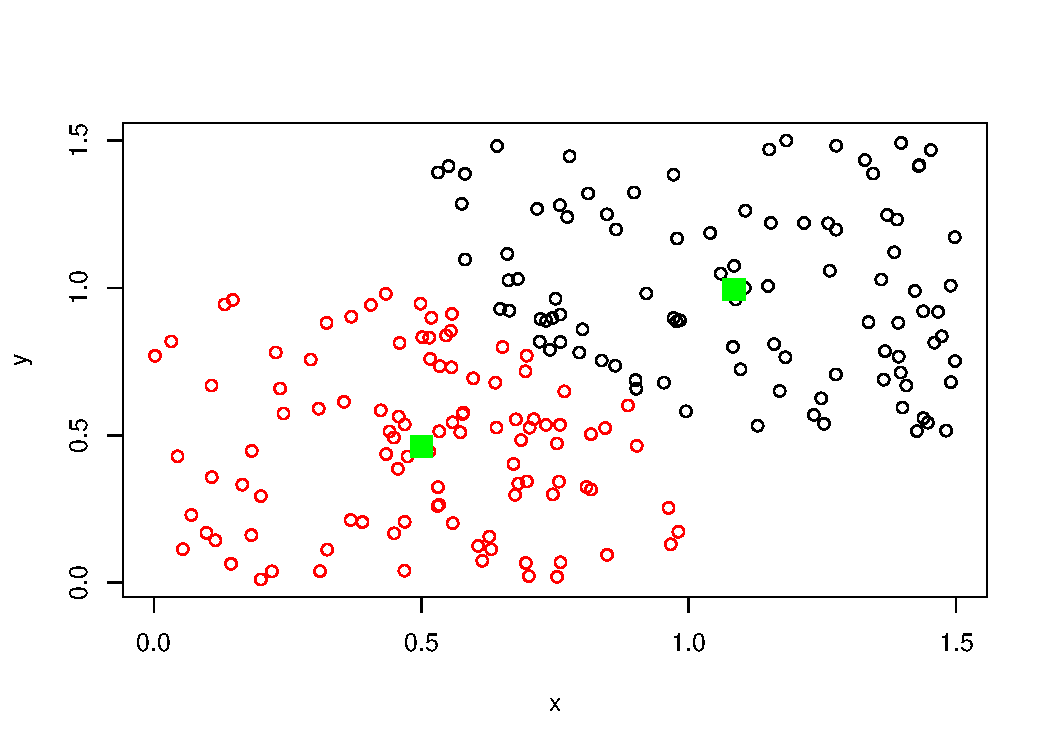
\includegraphics[width=\maxwidth]{figure/beamer-unnamed-chunk-4-1} 

}



\end{knitrout}
\end{frame}


\begin{frame}[fragile]{Linear Regression}
\begin{itemize}
\item We can use the {\tt lm} function for fitting a linear regression model:
\end{itemize}
\begin{knitrout}\footnotesize
\definecolor{shadecolor}{rgb}{0.969, 0.969, 0.969}\color{fgcolor}\begin{kframe}
\begin{alltt}
\hlstd{x} \hlkwb{=} \hlkwd{c}\hlstd{(}\hlnum{5}\hlstd{,} \hlnum{7}\hlstd{,} \hlnum{9}\hlstd{,} \hlnum{11}\hlstd{,} \hlnum{13}\hlstd{,} \hlnum{15}\hlstd{); y} \hlkwb{=} \hlkwd{c}\hlstd{(}\hlnum{11}\hlstd{,} \hlnum{14}\hlstd{,} \hlnum{20}\hlstd{,} \hlnum{24}\hlstd{,} \hlnum{29}\hlstd{,} \hlnum{31}\hlstd{)}
\hlcom{# stores the estimates of slope and y-intercept}
\hlstd{fit} \hlkwb{=} \hlkwd{lm}\hlstd{(y}\hlopt{~}\hlstd{x);} \hlkwd{class}\hlstd{(fit)} \hlcom{# of class "lm"}
\end{alltt}
\begin{verbatim}
## [1] "lm"
\end{verbatim}
\begin{alltt}
\hlkwd{predict}\hlstd{(fit)} \hlcom{# calculates the predicted y's (for the x's used in input)}
\end{alltt}
\begin{verbatim}
##        1        2        3        4        5        6 
## 10.85714 15.11429 19.37143 23.62857 27.88571 32.14286
\end{verbatim}
\begin{alltt}
\hlstd{y.int} \hlkwb{=} \hlstd{fit}\hlopt{$}\hlstd{coefficients[}\hlnum{1}\hlstd{]}
\hlstd{slope} \hlkwb{=} \hlstd{fit}\hlopt{$}\hlstd{coefficients[}\hlnum{2}\hlstd{]}
\end{alltt}
\end{kframe}
\end{knitrout}
\end{frame}

\begin{frame}[fragile]
A number of useful summaries are supplied by taking the {\tt summary()} on an \verb|"lm"| type object:
\begin{knitrout}\footnotesize
\definecolor{shadecolor}{rgb}{0.969, 0.969, 0.969}\color{fgcolor}\begin{kframe}
\begin{alltt}
\hlstd{sfit} \hlkwb{<-} \hlkwd{summary}\hlstd{(fit)}
\hlstd{sfit}\hlopt{$}\hlstd{r.squared} \hlcom{# R-squared value}
\end{alltt}
\begin{verbatim}
## [1] 0.9864919
\end{verbatim}
\begin{alltt}
\hlstd{sfit}\hlopt{$}\hlstd{residuals} \hlcom{# residuals}
\end{alltt}
\begin{verbatim}
##          1          2          3          4          5          6 
##  0.1428571 -1.1142857  0.6285714  0.3714286  1.1142857 -1.1428571
\end{verbatim}
\begin{alltt}
\hlstd{sfit}\hlopt{$}\hlstd{coefficients} \hlcom{# p-values/t-tests for parameter estimates}
\end{alltt}
\begin{verbatim}
##              Estimate Std. Error    t value     Pr(>|t|)
## (Intercept) 0.2142857   1.316044  0.1628256 8.785506e-01
## x           2.1285714   0.124540 17.0914722 6.873635e-05
\end{verbatim}
\end{kframe}
\end{knitrout}
\end{frame}


\begin{frame}[fragile]
Plotting is as simple as:
\begin{knitrout}\footnotesize
\definecolor{shadecolor}{rgb}{0.969, 0.969, 0.969}\color{fgcolor}\begin{kframe}
\begin{alltt}
\hlkwd{plot}\hlstd{(x, y,} \hlkwc{main}\hlstd{=}\hlstr{"Linear Regression Example"}\hlstd{)}
\hlkwd{abline}\hlstd{(fit,} \hlkwc{col}\hlstd{=}\hlstr{"blue"}\hlstd{)}
\end{alltt}
\end{kframe}

{\centering 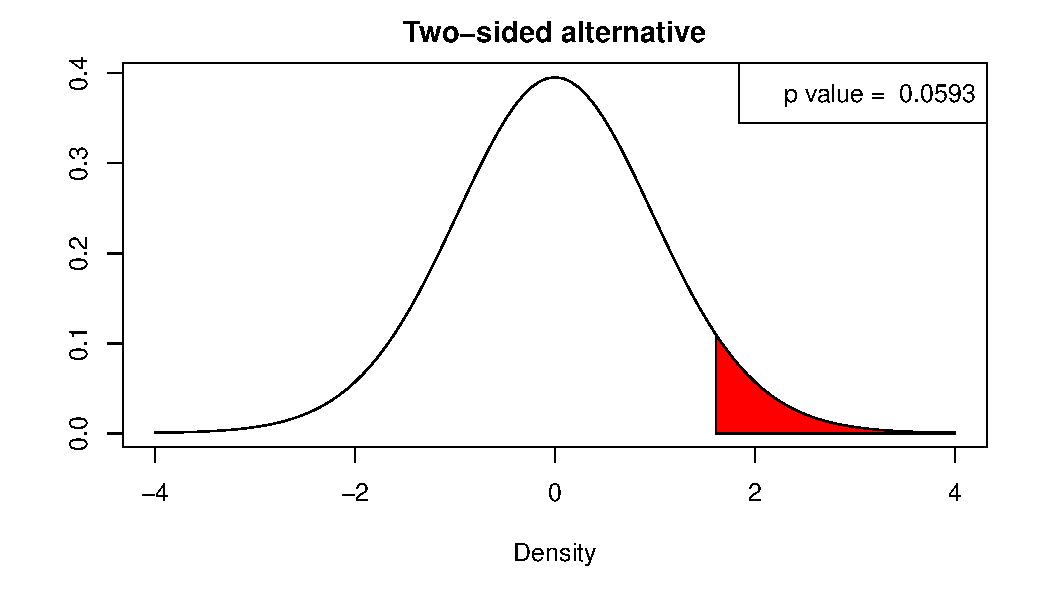
\includegraphics[width=\maxwidth]{figure/beamer-unnamed-chunk-7-1} 

}



\end{knitrout}
\end{frame}

\begin{frame}{Background}
\begin{itemize}
% \item One of the most important aspects of data analysis is the generation of proper graphics.
\item One of the main reasons data analysts turn to R is for its strong graphic capabilities.
\item R's model for constructing plots strikes a balance between structure and flexibilty. 
\item Base {\tt R} has a number of functions for basic plots which include:
\begin{itemize}
% \item Strip charts
\item Scatter plots
\item Histograms
\item Boxplots
\end{itemize}
\end{itemize}
\end{frame}



\begin{frame}[fragile]{Scatterplots}
\begin{itemize}
\item Plots of this type are produced using \rf{plot}\rt{(\rp x, \rp y, \rp{...})} in \R.
\vfill
\item The first argument supplies the $x$ co-ordinate values, while the second number provides the $y$ co-ordinate values.
\vfill
\item The \rp{...} denotes optional graphical parameters\footnote[frame]{see a nice summary of some useful ones \href{https://www.statmethods.net/advgraphs/parameters.html}{here} and a \href{https://www.gastonsanchez.com/r-graphical-parameters-cheatsheet.pdf}{cheat sheet}}
\begin{description}
\item[\rp{main}] A character string used in the title
\item[\rp{xlab}/\rp{ylab}] A character string used for the x/y axis labels
\item[\rp{xlim}/\rp{ylim}] A vector = {\tt c(xmin, xmax)}/{\tt c(ymin, ymax)} used for the plotting ranges
\item[\rp{cex}] number indicating  plotting text/symbols size. (1=default, 1.5 is 50\% larger, 0.5 is 50\% smaller, etc.)
\end{description}
\end{itemize}
\end{frame}

\begin{frame}[fragile]{Scatterplots}
\begin{knitrout}\footnotesize
\definecolor{shadecolor}{rgb}{0.969, 0.969, 0.969}\color{fgcolor}\begin{kframe}
\begin{alltt}
\hlstd{x} \hlkwb{=} \hlkwd{runif}\hlstd{(}\hlkwc{n}\hlstd{=}\hlnum{100}\hlstd{)} \hlcom{# 100 random numbers between 0 and 1}
\hlstd{y} \hlkwb{=} \hlkwd{runif}\hlstd{(}\hlkwc{n}\hlstd{=}\hlnum{100}\hlstd{,} \hlkwc{min}\hlstd{=}\hlnum{0}\hlstd{,} \hlkwc{max}\hlstd{=}\hlnum{5}\hlstd{)} \hlcom{# 100 random numbers between 0 and 5}
\hlkwd{plot}\hlstd{(x,y)}
\end{alltt}
\end{kframe}

{\centering 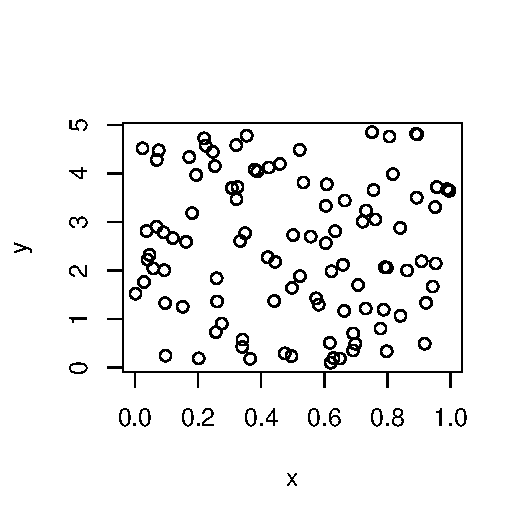
\includegraphics[width=0.4\textwidth]{figure/beamer-unnamed-chunk-8-1} 

}



\end{knitrout}
\end{frame}


\begin{frame}{Histograms}
\begin{itemize}
\item A histogram is very common visualization that plots the %frequencies that data appears within certain ranges. 
number of observations  appearing within certain ranges called ``bins".
\item Bins (or ``buckets") are constructed by dividing the entire range of values into a series of intervals.%—and then count how many values fall into each interval. 
\item In \R histograms are produced using the \rf{hist}\rt{()} function
\item \rf{hist}\rt{()} tries to calculate reasonable bins automatically; however, we can manually set them ourselves in the \rp{breaks} argument
\end{itemize}
\end{frame}


\begin{frame}[fragile]{}
\begin{knitrout}\footnotesize
\definecolor{shadecolor}{rgb}{0.969, 0.969, 0.969}\color{fgcolor}\begin{kframe}
\begin{alltt}
\hlstd{x} \hlkwb{=} \hlkwd{runif}\hlstd{(}\hlkwc{n}\hlstd{=}\hlnum{100}\hlstd{,} \hlkwc{min}\hlstd{=}\hlnum{1}\hlstd{,} \hlkwc{max} \hlstd{=}\hlnum{10}\hlstd{)}
\hlkwd{hist}\hlstd{(x)}
\end{alltt}
\end{kframe}

{\centering 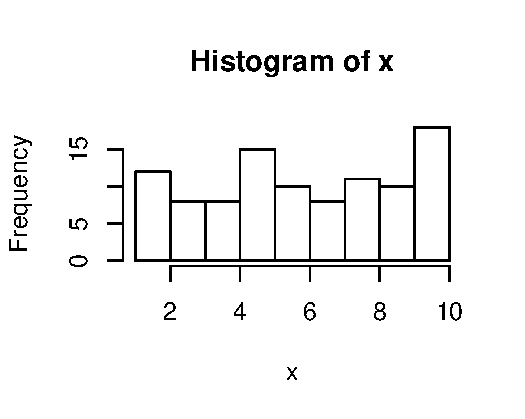
\includegraphics[width=\maxwidth]{figure/beamer-unnamed-chunk-9-1} 

}



\end{knitrout}
\end{frame}

\begin{frame}[fragile]{}
\begin{knitrout}\footnotesize
\definecolor{shadecolor}{rgb}{0.969, 0.969, 0.969}\color{fgcolor}\begin{kframe}
\begin{alltt}
\hlstd{x} \hlkwb{=} \hlkwd{runif}\hlstd{(}\hlkwc{n}\hlstd{=}\hlnum{100}\hlstd{,} \hlkwc{min}\hlstd{=}\hlnum{1}\hlstd{,} \hlkwc{max} \hlstd{=}\hlnum{10}\hlstd{)}
\hlkwd{hist}\hlstd{(x,} \hlkwc{breaks} \hlstd{=} \hlnum{40}\hlstd{)}
\end{alltt}
\end{kframe}

{\centering 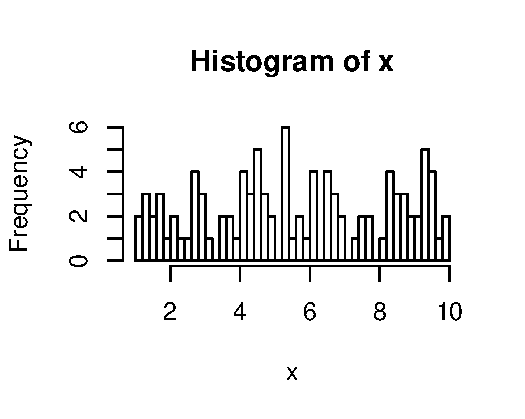
\includegraphics[width=\maxwidth]{figure/beamer-unnamed-chunk-10-1} 

}



\end{knitrout}
\end{frame}




\begin{frame}[fragile]{Boxplots}

\begin{itemize}
\item A boxplot (AKA box-and-whisker plot) provides a graphical view of the median, quartiles, maximum, and minimum of a data set (i.e. the five number summary). 
\vfill
\item When applicable, it will identify outliers and their values. 
\begin{itemize}
\item Outliers are defined to be $\geq Q3 + 1.5*$IQR or $\leq Q1 - 1.5*$IQR
\item Not all data will have outliers.
\end{itemize}
\vfill
 \item Boxplots provide a useful snapshot of your data and can indicate if  data is symmetric or skewed, for example.
 \vfill
 \item Beware that they can be misleading when there are very few data points %(in which case we should probably use a strip chart).
\end{itemize}
\end{frame}


 
 \begin{frame}{Boxplot}\label{labelboxplotSlide}
 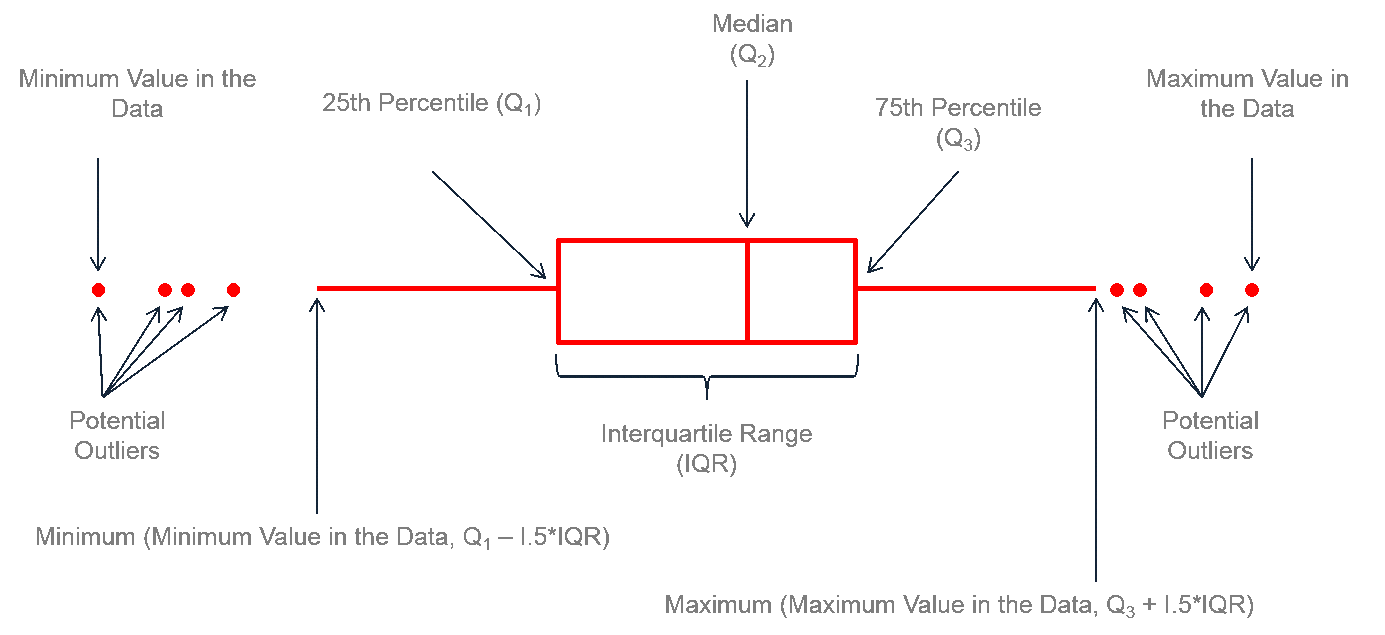
\includegraphics[width = 0.99\textwidth]{figure/boxplot.png}\\
 Image \href{https://www.leansigmacorporation.com/box-plot-with-minitab/}{source}
 \end{frame}


\begin{frame}[fragile]{Boxplots}
These plots are available through the \rf{boxplot()} command.

\begin{knitrout}\footnotesize
\definecolor{shadecolor}{rgb}{0.969, 0.969, 0.969}\color{fgcolor}\begin{kframe}
\begin{alltt}
\hlstd{x} \hlkwb{<-} \hlkwd{rnorm}\hlstd{(}\hlnum{100}\hlstd{)} \hlcom{# generate 100 obs from a standard normal dist}
\hlkwd{boxplot}\hlstd{(x)}
\end{alltt}
\end{kframe}

{\centering 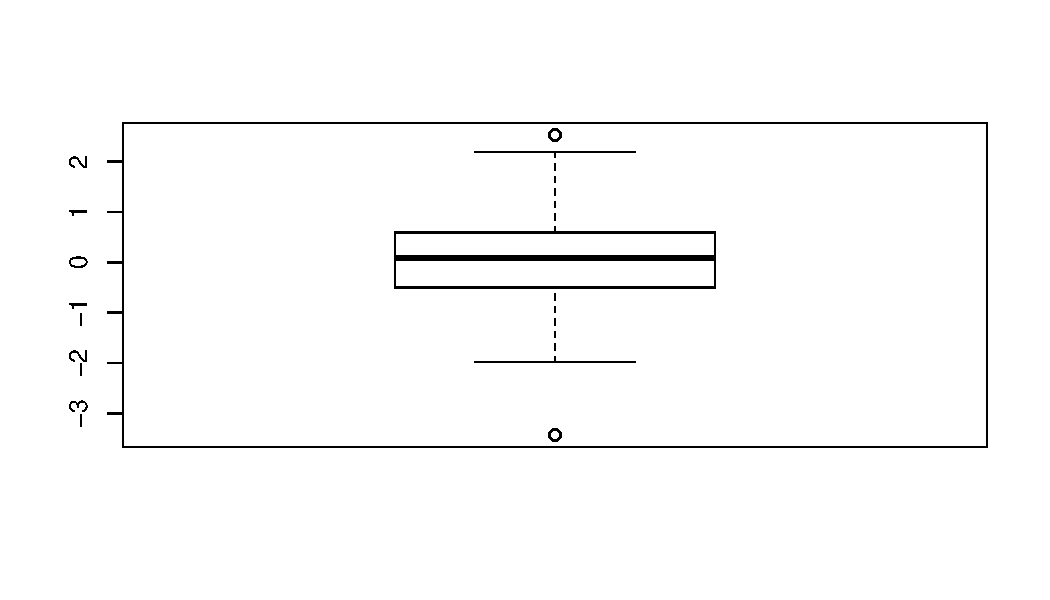
\includegraphics[width=\maxwidth]{figure/beamer-unnamed-chunk-12-1} 

}



\end{knitrout}
\end{frame}

\begin{frame}[fragile]{Boxplots}
We can plot data horizontally by setting \rp{horizontal}=\rv{TRUE}
\begin{knitrout}\footnotesize
\definecolor{shadecolor}{rgb}{0.969, 0.969, 0.969}\color{fgcolor}\begin{kframe}
\begin{alltt}
\hlkwd{boxplot}\hlstd{(x,} \hlkwc{horizontal}\hlstd{=}\hlnum{TRUE}\hlstd{)}
\end{alltt}
\end{kframe}

{\centering 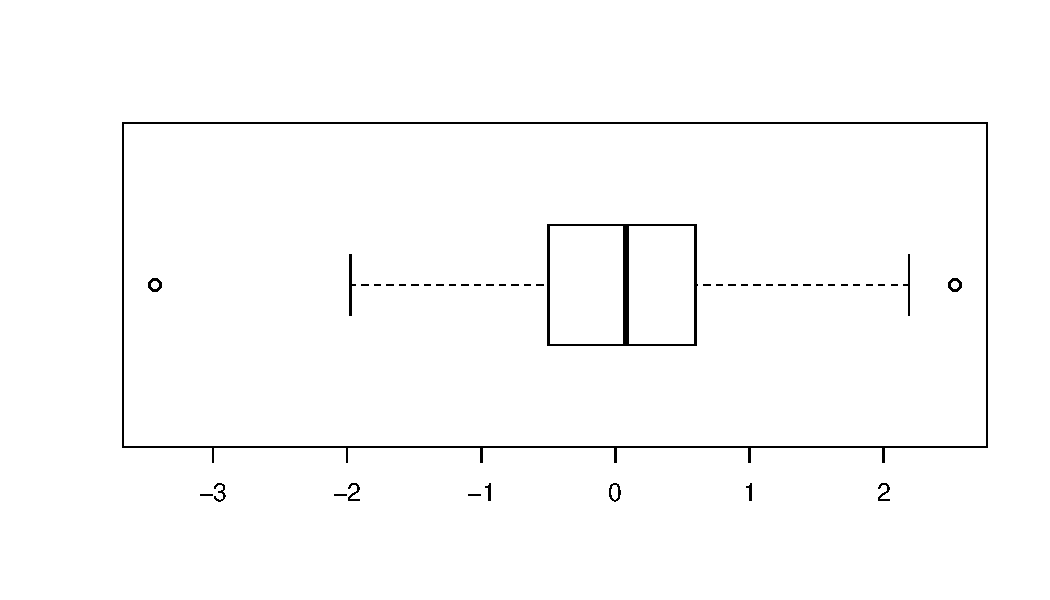
\includegraphics[width=\maxwidth]{figure/beamer-unnamed-chunk-13-1} 

}



\end{knitrout}
\end{frame}



\begin{frame}[fragile]{Boxplots}
\begin{itemize}
\item The ``box" portion represents the IQR  = Q3 - Q1.
\vfill
\item The line near the middle represents the median (i.e. Q2). 
\vfill
\item  The points on the edge of the plot are potential outliers
\begin{itemize}
\item Recall outliers are $\geq Q3 + 1.5*$IQR or $\leq Q1 - 1.5*$IQR
\item Not all data will have outliers.
\end{itemize}
\vfill
\item The ends of the ``whiskers" represent the maximum and minimum observation that are not considered outliers.
\end{itemize}
\end{frame}

\begin{frame}[fragile]{Adding lines to a plot}
\begin{itemize}
\item  To varify that these markings correspond  with the five number summary, we can use \rf{abline}.  
\vfill
\item \rf{abline} adds a line to the current plot by either specifying:\footnote[frame]{it can also take an {\tt lm} object as an argument}  a slope (\rp a) and $y$-intercept (\rp b); a single $y$-value (\rp h) for drawing a horizontal line; a single $x$-value (\rp v) for drawing a vertical line
\vfill
\item Related functions:
\begin{description}
\item[\rf{points}\rt{()}] for adding points to the current graph
\item[\rf{text}\rt{()}] for adding text to the current graph
\end{description}
\vfill
\end{itemize}
\end{frame}

\begin{frame}[fragile]{Adding Lines to a Plot}
\begin{knitrout}\footnotesize
\definecolor{shadecolor}{rgb}{0.969, 0.969, 0.969}\color{fgcolor}\begin{kframe}
\begin{alltt}
\hlstd{x5} \hlkwb{=} \hlkwd{fivenum}\hlstd{(x);} \hlkwd{names}\hlstd{(x5)} \hlkwb{=} \hlkwd{c}\hlstd{(}\hlstr{"min"}\hlstd{,}\hlstr{"q1"}\hlstd{,}\hlstr{"median"}\hlstd{,}\hlstr{"q3"}\hlstd{,}\hlstr{"max"}\hlstd{)}
\hlkwd{boxplot}\hlstd{(x)}
\hlcom{# Draw a red dashed line at Q1}
\hlkwd{abline}\hlstd{(}\hlkwc{h}\hlstd{=x5[}\hlstr{"q1"}\hlstd{],} \hlkwc{col}\hlstd{=}\hlnum{2}\hlstd{,} \hlkwc{lty}\hlstd{=}\hlnum{2}\hlstd{)}
\hlcom{# Draw a green thick line at Q2 (the median)}
\hlkwd{abline}\hlstd{(}\hlkwc{h}\hlstd{=x5[}\hlstr{"median"}\hlstd{],} \hlkwc{col}\hlstd{=}\hlstr{"green"}\hlstd{,} \hlkwc{lwd} \hlstd{=} \hlnum{3}\hlstd{)}
\hlcom{# Draw a purple dotted line at Q3}
\hlkwd{abline}\hlstd{(}\hlkwc{h}\hlstd{=x5[}\hlstr{"q3"}\hlstd{],} \hlkwc{col}\hlstd{=}\hlstr{"purple"}\hlstd{,} \hlkwc{lty} \hlstd{=} \hlnum{3}\hlstd{)}
\end{alltt}
\end{kframe}
\end{knitrout}
\end{frame}



\begin{frame}[fragile]{}
\begin{knitrout}\footnotesize
\definecolor{shadecolor}{rgb}{0.969, 0.969, 0.969}\color{fgcolor}

{\centering 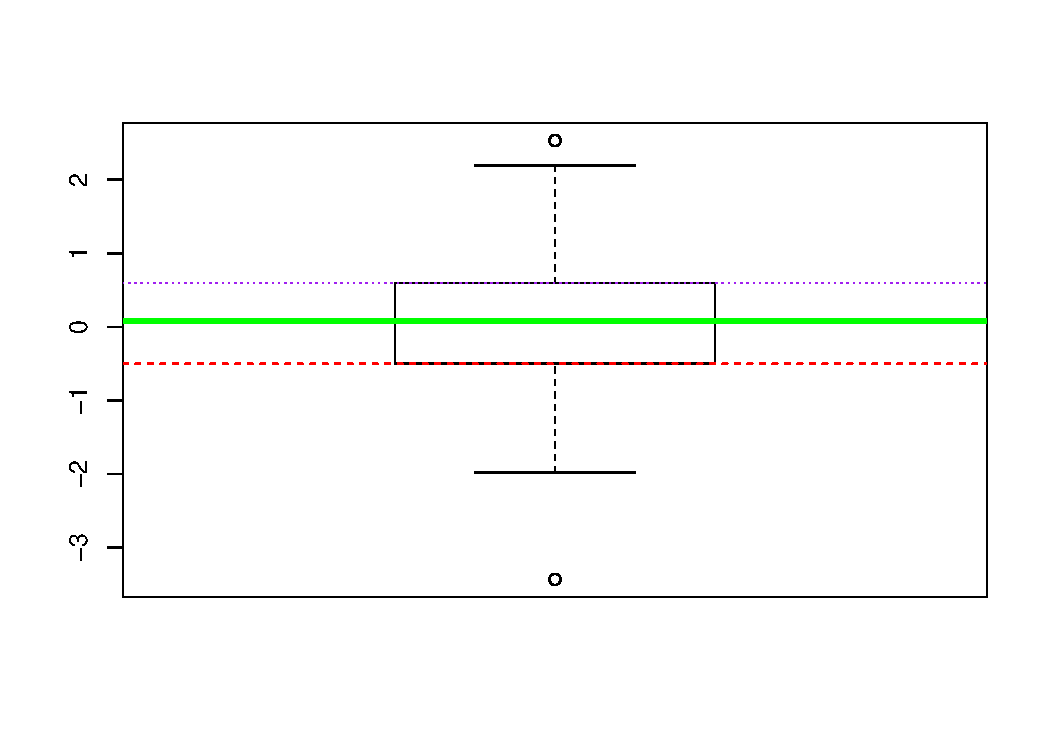
\includegraphics[width=\maxwidth]{figure/beamer-xboxplot-1} 

}



\end{knitrout}

\end{frame}

\begin{frame}[fragile]{R colours}
We can used colour indeces instead of colour names, eg. 2 = red. 
\begin{knitrout}\footnotesize
\definecolor{shadecolor}{rgb}{0.969, 0.969, 0.969}\color{fgcolor}\begin{kframe}
\begin{alltt}
\hlkwd{palette}\hlstd{()} \hlcom{# See the entire colour palette}
\end{alltt}
\begin{verbatim}
## [1] "black"   "red"     "green3"  "blue"    "cyan"    "magenta" "yellow" 
## [8] "gray"
\end{verbatim}
\begin{alltt}
\hlkwd{palette}\hlstd{()[}\hlnum{2}\hlstd{]} \hlcom{# colour index 2 = red}
\end{alltt}
\begin{verbatim}
## [1] "red"
\end{verbatim}
\end{kframe}
\end{knitrout}
See \href{http://www.stat.columbia.edu/~tzheng/files/Rcolor.pdf}{here} for the list of available colour names in {\tt R}
\end{frame}

\begin{frame}[fragile]{Boxplot deconstruction}
\begin{itemize}
\item To determine where our whiskers end, we first need to find our cut-off for potential outliers:
\begin{knitrout}\footnotesize
\definecolor{shadecolor}{rgb}{0.969, 0.969, 0.969}\color{fgcolor}\begin{kframe}
\begin{alltt}
\hlstd{IQR} \hlkwb{=} \hlstd{x5[}\hlstr{"q3"}\hlstd{]} \hlopt{-} \hlstd{x5[}\hlstr{"q1"}\hlstd{]}
\hlstd{upper} \hlkwb{=} \hlstd{x5[}\hlstr{"q3"}\hlstd{]} \hlopt{+} \hlnum{1.5}\hlopt{*}\hlstd{IQR}
\hlstd{lower} \hlkwb{=} \hlstd{x5[}\hlstr{"q1"}\hlstd{]} \hlopt{-} \hlnum{1.5}\hlopt{*}\hlstd{IQR}
\hlstd{(outliers} \hlkwb{=} \hlkwd{c}\hlstd{(}\hlkwd{which}\hlstd{(x}\hlopt{>}\hlstd{upper} \hlopt{|} \hlstd{x}\hlopt{<}\hlstd{lower)))}
\end{alltt}
\begin{verbatim}
## [1] 33 46
\end{verbatim}
\begin{alltt}
\hlstd{x[outliers]}
\end{alltt}
\begin{verbatim}
## [1]  2.530865 -3.431558
\end{verbatim}
\end{kframe}
\end{knitrout}
\end{itemize}
\end{frame}

\begin{frame}[fragile]{Boxplot deconstruction}
\begin{itemize}
\item The whiskers end at the min and max values in the data with the  outliers removed.
\begin{knitrout}\footnotesize
\definecolor{shadecolor}{rgb}{0.969, 0.969, 0.969}\color{fgcolor}\begin{kframe}
\begin{alltt}
\hlstd{minx} \hlkwb{=} \hlkwd{min}\hlstd{(x[}\hlopt{-}\hlstd{outliers])}
\hlstd{maxx} \hlkwb{=} \hlkwd{max}\hlstd{(x[}\hlopt{-}\hlstd{outliers])}
\end{alltt}
\end{kframe}
\end{knitrout}
\item Adding these values to the plot from before we get:
\begin{knitrout}\footnotesize
\definecolor{shadecolor}{rgb}{0.969, 0.969, 0.969}\color{fgcolor}\begin{kframe}
\begin{alltt}
\hlkwd{abline}\hlstd{(}\hlkwc{h}\hlstd{=minx,} \hlkwc{col}\hlstd{=}\hlstr{"blue"}\hlstd{)}
\hlkwd{abline}\hlstd{(}\hlkwc{h}\hlstd{=maxx,} \hlkwc{col}\hlstd{=}\hlstr{"gold"}\hlstd{)}
\hlcom{# plot the outlines in big blue triangles (pch = 2)}
\hlkwd{points}\hlstd{(x[outliers][}\hlnum{1}\hlstd{],} \hlkwc{col}\hlstd{=}\hlstr{"dodgerblue2"}\hlstd{,} \hlkwc{cex}\hlstd{=}\hlnum{3}\hlstd{,} \hlkwc{pch} \hlstd{=}\hlnum{2}\hlstd{)}
\hlkwd{points}\hlstd{(x[outliers][}\hlnum{2}\hlstd{],} \hlkwc{col}\hlstd{=}\hlstr{"dodgerblue2"}\hlstd{,} \hlkwc{cex}\hlstd{=}\hlnum{3}\hlstd{,} \hlkwc{pch} \hlstd{=}\hlnum{2}\hlstd{)}
\end{alltt}
\end{kframe}
\end{knitrout}
\end{itemize}
\end{frame}

\begin{frame}[fragile]{}
\begin{knitrout}\footnotesize
\definecolor{shadecolor}{rgb}{0.969, 0.969, 0.969}\color{fgcolor}

{\centering 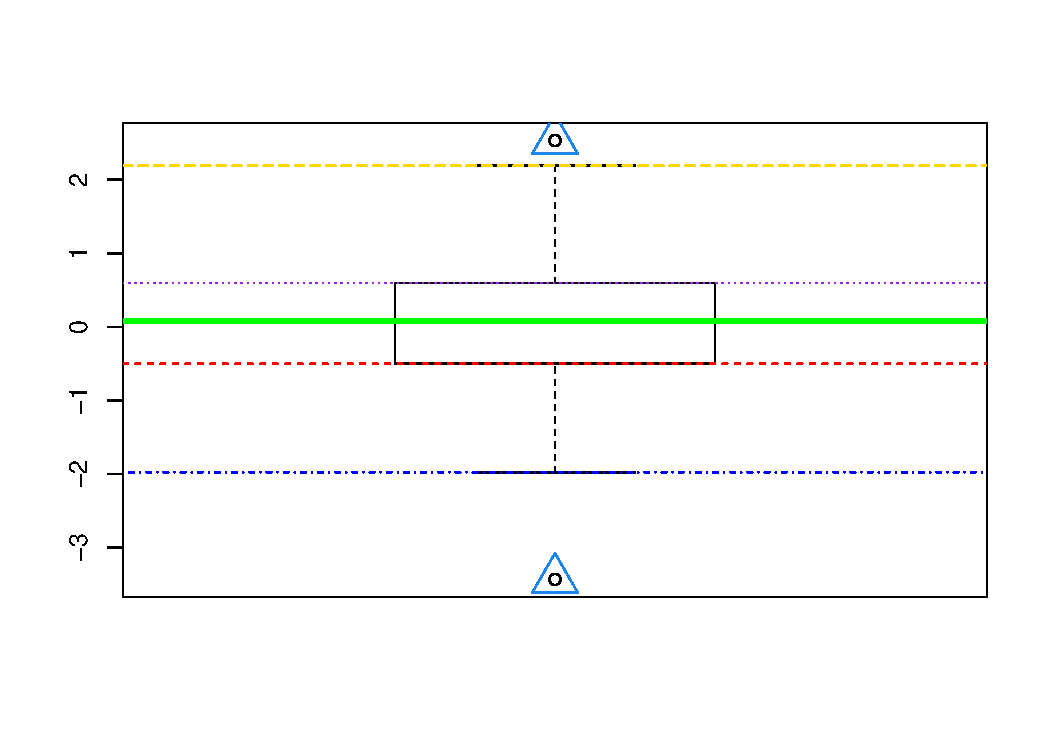
\includegraphics[width=\maxwidth]{figure/beamer-unnamed-chunk-19-1} 

}



\end{knitrout}
Note that we can only add (not take away) markings in base plotting
\end{frame}




\begin{frame}[fragile]{Visualizing Data in R}
\begin{itemize}
\item R supports several graphing \emph{libraries} (i.e. packages) for producing graphics.
\vfill
\item One of the most popular packages for plotting is \rt{ggplot2} written by Hadley Wickham.
\vfill
% \item \verb|gg| stands for Grammar of Graphics.
% \vfill
% \item See the \href{https://www.rstudio.com/wp-content/uploads/2015/03/ggplot2-cheatsheet.pdf}{\red{ggplot cheatsheet}}
\item \rt{ggplot2} implements the  \href{https://www.springer.com/gp/book/9780387245447}{\emph{Grammar of Graphics}} and enables us to concisely describe the components of a graphic. 
 \vfill
\item There is a lot to unpack with this graphic method and it may be helpful to keep a \href{https://www.rstudio.com/wp-content/uploads/2015/03/ggplot2-cheatsheet.pdf}{{cheatsheet}} nearby.
\vfill
\item Another great resource is the \href{https://ggplot2.tidyverse.org/}{ggplot2 website} and \href{https://ggplot2.tidyverse.org/reference/}{reference}.\end{itemize}
\end{frame}



\begin{frame}{What is an \R package?}
\begin{itemize}
\item Recall that an \R package is a sharable collection of code/data/functions/documentation.
\item While anyone can write a package and share, the Comprehensive R Archive Network, or CRAN is the main repository for vetted \R packages that meet a \href{https://cran.r-project.org/web/packages/policies.html}{\underline{specific criteria}}. 
\item  There is huge variety of packages  available on CRAN ($>$10000) and throughout this course we will be making use of a very small subset of them.
\end{itemize}
\end{frame}



\begin{frame}[fragile]{Installing \rt{ggplot2}}

To install \texttt{Tools $\to$ Install Packages}\ldots Then input \verb|ggplot2|.
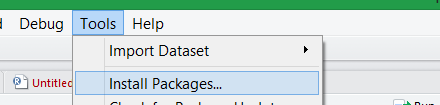
\includegraphics[width=0.5\textwidth]{img/debug}
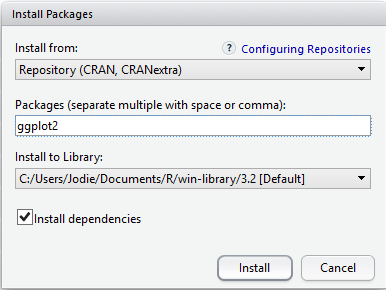
\includegraphics[width=.4\textwidth]{img/installpackage}

Alternatively (and this would be my preferred method) type the command:
\begin{knitrout}\footnotesize
\definecolor{shadecolor}{rgb}{0.969, 0.969, 0.969}\color{fgcolor}\begin{kframe}
\begin{alltt}
\hlkwd{install.packages}\hlstd{(}\hlstr{"ggplot2"}\hlstd{)}
\end{alltt}
\end{kframe}
\end{knitrout}
\end{frame}


\begin{frame}[fragile]{Installing \rt{ggplot2}}
To install this package from CRAN, load the package into \R, and access the help files, type the following:
\begin{knitrout}\footnotesize
\definecolor{shadecolor}{rgb}{0.969, 0.969, 0.969}\color{fgcolor}\begin{kframe}
\begin{alltt}
\hlcom{# install.packages("ggplot2") # install (only do once)}
\hlkwd{library}\hlstd{(}\hlstr{"ggplot2"}\hlstd{)}            \hlcom{# load}
\hlstd{package}\hlopt{?}\hlstd{ggplot2}               \hlcom{# help   }
\hlkwd{help}\hlstd{(}\hlkwc{package} \hlstd{=} \hlstr{"ggplot2"}\hlstd{)}     \hlcom{# another way to get help}
\end{alltt}
\end{kframe}
\end{knitrout}
\end{frame}

\begin{frame}[fragile]{A note on installing packages}
\begin{itemize}
\item Note that this install need only be done once on your personal computer (if you are running this on the lab computers you may need to reinstall every time you log on). 
\vfill
\item The {\tt library("ggplot2")} command will need to be executed at each new \R session, i.e. every time you close and reopen \R Studio
\vfill
\end{itemize}
\end{frame}



\begin{frame}{Grammar of Graphics}
Some notation
\begin{description}
\item[aes] aesthetic attributes, i.e. how data are mapped (eg. colour, shape, size)
\item[geoms] geometric objects (eg. points, lines, bars).  Also referred to as \textit{layers}.  See \href{https://ggplot2.tidyverse.org/reference/}{here} for all available geoms.
\item[facets] for forming multi-panel plots
\item[stats] for statistical transformation (eg. smoothing) %rather than the visual appearance.
% \item[scales] used for aesthetic mappings
\item[co-ordinate system] (eg. $x$ and $y$ axis)
\end{description}
\end{frame}

% cool graphics in base: https://flowingdata.com/2016/03/22/comparing-ggplot2-and-r-base-graphics/



\begin{frame}[fragile]{The basics of \rt{ggplot2}}
\begin{itemize}
\item \rf{ggplot()} is the workhorse function in \rt{ggplot2}.
\vfill
\item \rf{ggplot()}  works similar to the {\bf base} plotting system, in that we can overlay layers and build-up our plot.
\vfill
\item Rather than specifying graphical features of our plot with \rp{arguments} in a \rf{function}, we will add them (literally by using {\tt +}) to a {\tt ggplot} \emph{object}.% layer by layer.
\end{itemize}
\end{frame}




\begin{frame}[fragile]{General workflow:}
\begin{itemize}
\item Identify your data and basic aestheics (identify $x$ and $y$ variables for example)
\begin{itemize}
\item I'm using the \ro{mtcars} dataset (see {\tt ?mtcars})
\item To produce a simple 2D scatterplot I need to identify which variable will be plotted on the $x$-axis and $y$-axis (note that there are 11 variables in this dataset)
\end{itemize}

\item Save this to an \R \textit{object} (which will be {\tt ggplot} \textit{class}). 
\vfill
\item Standard convention is to call this ggplot object \ro{g}.
% \item Pro tip: organizing you data and meta-data,(eg. column names) before you start plotting is going to make coding much simpler.
\vfill
\end{itemize}
\end{frame}



\begin{frame}[fragile]{General workflow:}
\begin{knitrout}\footnotesize
\definecolor{shadecolor}{rgb}{0.969, 0.969, 0.969}\color{fgcolor}\begin{kframe}
\begin{alltt}
\hlkwd{library}\hlstd{(ggplot2)}
\end{alltt}


{\ttfamily\noindent\color{warningcolor}{\#\# Warning: As of rlang 0.4.0, dplyr must be at least version 0.8.0.\\\#\# x dplyr 0.7.7 is too old for rlang 0.4.1.\\\#\# i Please update dplyr with `install.packages("{}dplyr"{})`.}}\begin{alltt}
\hlstd{g} \hlkwb{=} \hlkwd{ggplot}\hlstd{(mtcars,} \hlkwd{aes}\hlstd{(}\hlkwc{x}\hlstd{=mpg,} \hlkwc{y}\hlstd{=disp))} \hlcom{# identify data and x/y variables}
\hlkwd{class}\hlstd{(g)}
\end{alltt}
\begin{verbatim}
## [1] "gg"     "ggplot"
\end{verbatim}
\end{kframe}
\end{knitrout}
Note that there is nothing plotted when we create this object
\end{frame}



\begin{frame}[fragile]{General workflow:}
Create desired layers, some examples:
\begin{itemize}
\item \rt{geom\_point()} creates geometric points
\item \rt{geom\_smooth()} creates a smoother
\begin{itemize}
\item \rt{geom\_smooth(method="lm")} creates a regression line.
\end{itemize}
\item \rt{facet\_grid()} for multi-panel plots
\item \rt{theme\_bw()} changes gray background to black and white theme. 
\item \dots, many more (see \href{https://www.rstudio.com/wp-content/uploads/2015/03/ggplot2-cheatsheet.pdf}{cheatsheet})
\end{itemize}
\end{frame}


\begin{frame}[fragile]{Scatterplot}
Like \rt{plot(mpg, disp, data=mtcars)} in {\bf base}
\begin{knitrout}\footnotesize
\definecolor{shadecolor}{rgb}{0.969, 0.969, 0.969}\color{fgcolor}\begin{kframe}
\begin{alltt}
\hlstd{g} \hlopt{+} \hlkwd{geom_point}\hlstd{()}
\end{alltt}
\end{kframe}

{\centering 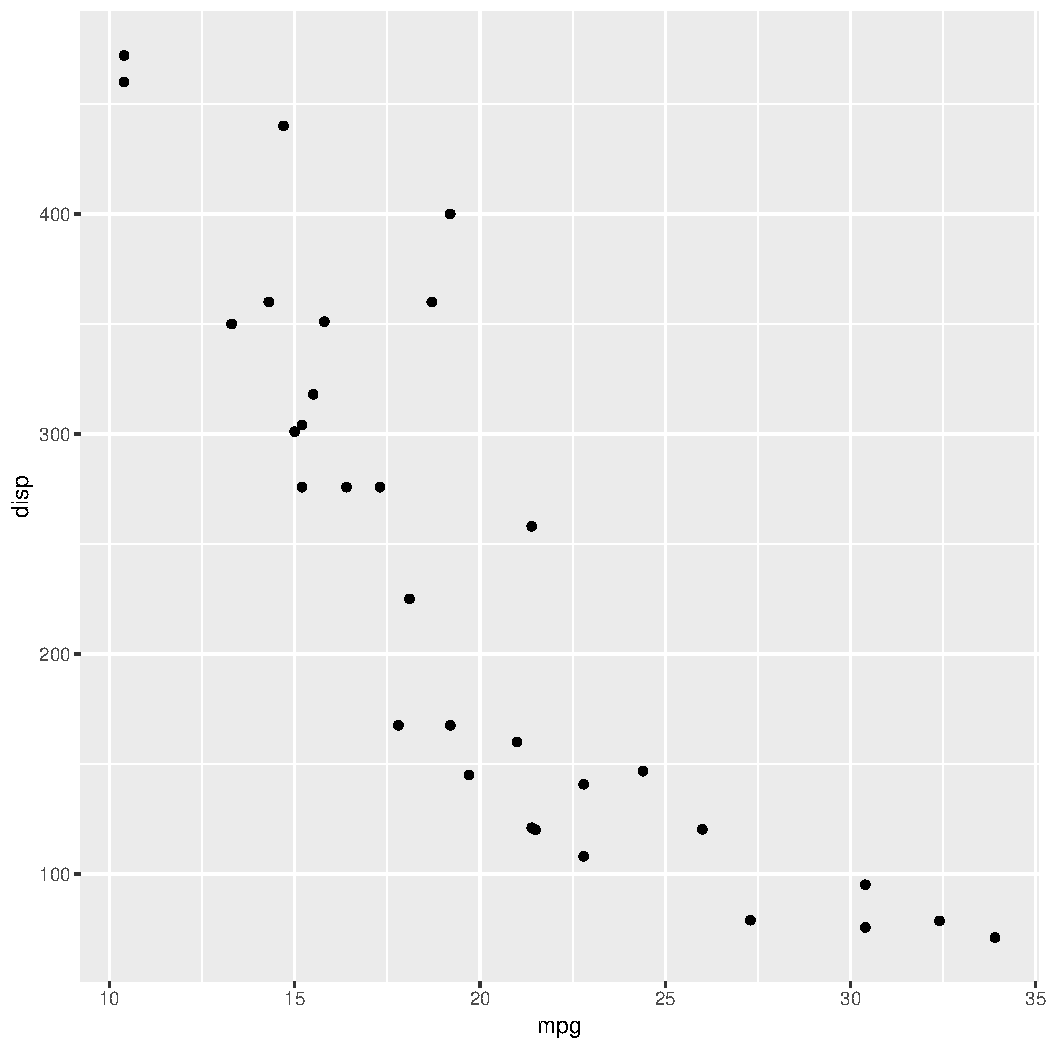
\includegraphics[width=0.5\linewidth]{figure/beamer-unnamed-chunk-22-1} 

}



\end{knitrout}
\end{frame}


\begin{frame}[fragile]{Adding a line}
Add a line overtop our scatterplot (similar to \rf{abline()} in {\bf base}). 
\begin{knitrout}\footnotesize
\definecolor{shadecolor}{rgb}{0.969, 0.969, 0.969}\color{fgcolor}\begin{kframe}
\begin{alltt}
\hlstd{g} \hlopt{+} \hlkwd{geom_point}\hlstd{()} \hlopt{+} \hlkwd{geom_smooth}\hlstd{(}\hlkwc{method} \hlstd{=}\hlstr{"lm"}\hlstd{)}
\end{alltt}
\end{kframe}

{\centering 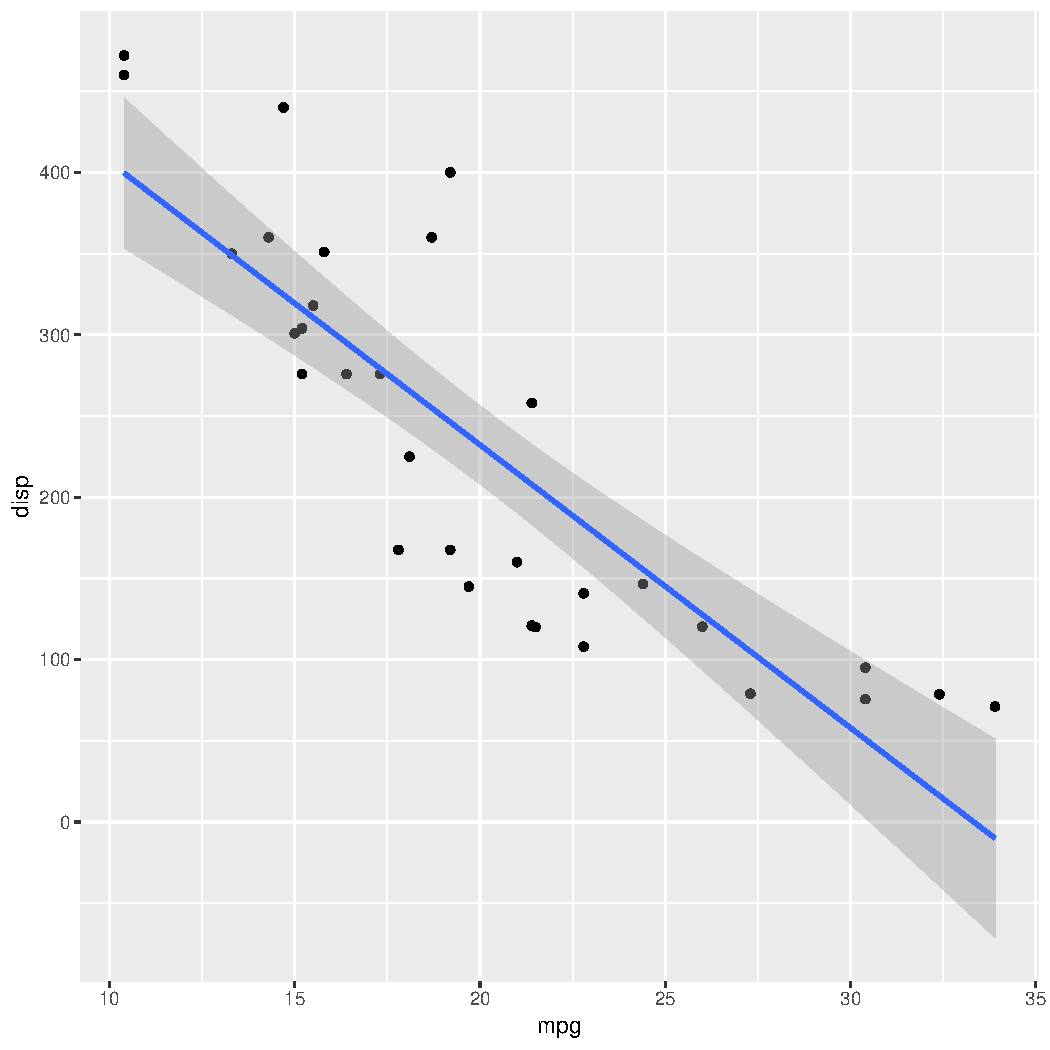
\includegraphics[width=0.5\linewidth]{figure/beamer-unnamed-chunk-23-1} 

}



\end{knitrout}
\end{frame}


\begin{frame}[fragile]{Change Theme}
Change the theme from gray to black and white.
\begin{knitrout}\footnotesize
\definecolor{shadecolor}{rgb}{0.969, 0.969, 0.969}\color{fgcolor}\begin{kframe}
\begin{alltt}
\hlstd{g} \hlopt{+} \hlkwd{geom_point}\hlstd{()} \hlopt{+} \hlkwd{theme_bw}\hlstd{()}
\end{alltt}
\end{kframe}

{\centering 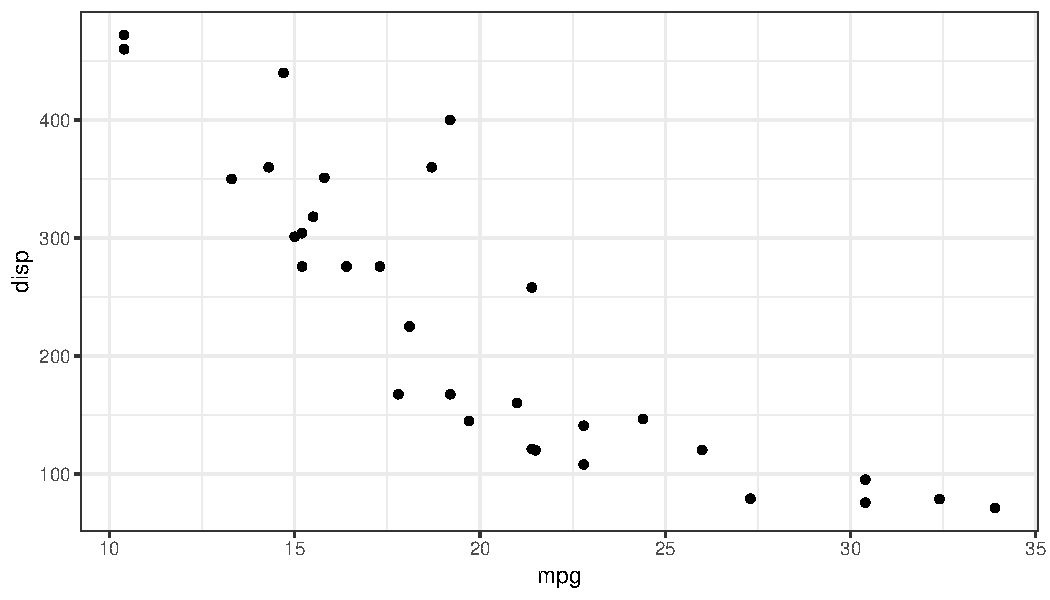
\includegraphics[width=0.8\linewidth]{figure/beamer-unnamed-chunk-24-1} 

}



\end{knitrout}
\end{frame}



\begin{frame}[fragile]{Adjusting Graphical Parameters}
\begin{itemize}
\item Annotate with meta-data:
\begin{itemize}
\item Change labels using \rf{xlab()}, \rf{ylab()}, \rf{ggtitle()}, or \rf{labs()} (which is a more general can specify x,y,title)
\begin{itemize}
\item \rt{labs(\rp{x}=<>, \rp{y}=<>, \rp{title}<>)}
\end{itemize}
\end{itemize}
\item Manage {\bf geom} obects. For example change the default settings in  {geom\_point}
\begin{itemize}
\item \rt{geom\_point(\rp{color}=<>, \rp{size}=<>, \rp{alpha} =<>)}
\item where {\tt alpha} controls the transparency (0 for completely transparent, 1 for completely opaque)
\item see more options \href{https://ggplot2.tidyverse.org/reference/geom_point.html}{here}
\end{itemize}
\end{itemize}
\end{frame}



\begin{frame}[fragile]{}
\begin{knitrout}\footnotesize
\definecolor{shadecolor}{rgb}{0.969, 0.969, 0.969}\color{fgcolor}\begin{kframe}
\begin{alltt}
\hlkwd{ggplot}\hlstd{(mtcars,} \hlkwd{aes}\hlstd{(}\hlkwc{x}\hlstd{=mpg,} \hlkwc{y}\hlstd{=disp))} \hlopt{+} \hlkwd{geom_point}\hlstd{(}\hlkwc{color}\hlstd{=}\hlstr{'darkblue'}\hlstd{)}
\end{alltt}
\end{kframe}

{\centering 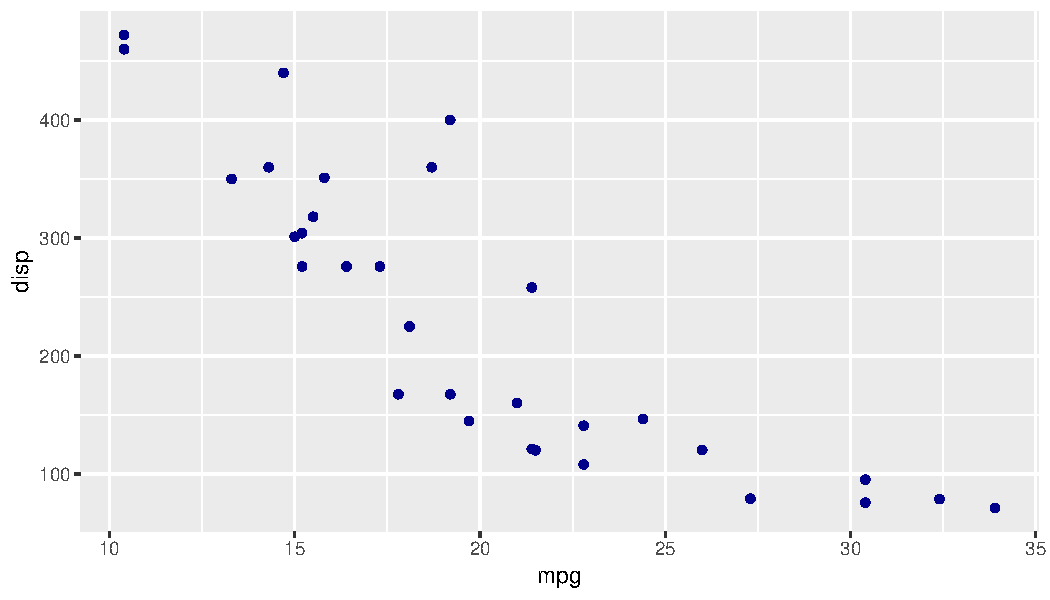
\includegraphics[width=0.8\linewidth]{figure/beamer-unnamed-chunk-25-1} 

}



\end{knitrout}
Note here that I am calling \rf{ggplot} directly and not saving a ggplot object
\end{frame}


\begin{frame}[fragile]{}
\begin{knitrout}\footnotesize
\definecolor{shadecolor}{rgb}{0.969, 0.969, 0.969}\color{fgcolor}\begin{kframe}
\begin{alltt}
\hlstd{g} \hlopt{+} \hlkwd{geom_point}\hlstd{(}\hlkwc{color}\hlstd{=}\hlstr{'darkblue'}\hlstd{,} \hlkwc{size} \hlstd{=} \hlnum{5}\hlstd{,} \hlkwc{alpha} \hlstd{=} \hlnum{0.3}\hlstd{)}
\end{alltt}
\end{kframe}

{\centering 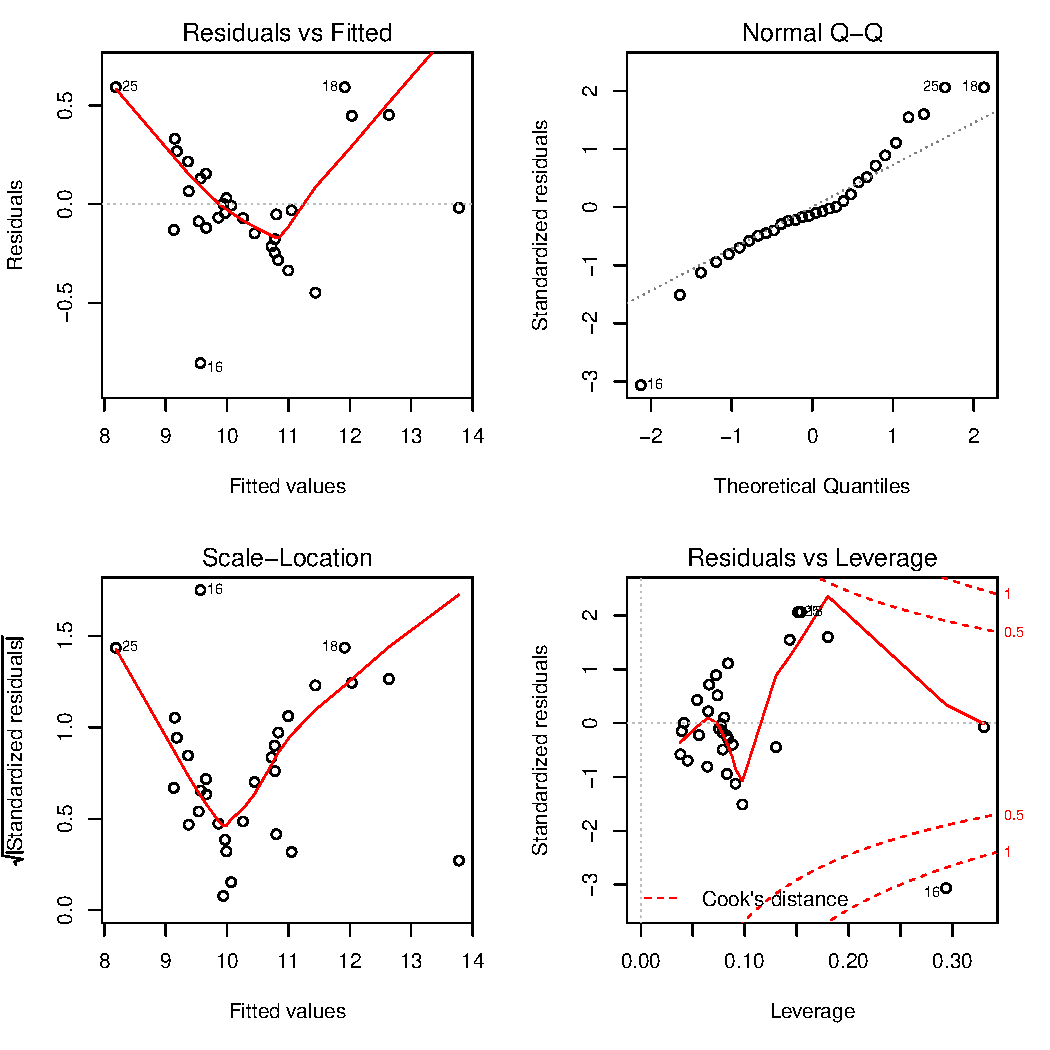
\includegraphics[width=0.8\linewidth]{figure/beamer-unnamed-chunk-26-1} 

}



\end{knitrout}
Notice how overlapping points are more obvious when using semi-transparent points.
\end{frame}



\begin{frame}[fragile]{}
\begin{itemize}
\item We can also colour points according to some  category (a factor type variable). 
\vfill
\item Notice how we do not need to specify colours and legends in \ggplot (although we could change the default settings if we wanted to see \href{http://www.sthda.com/english/wiki/ggplot2-colors-how-to-change-colors-automatically-and-manually}{here})
\vfill
\item Notice how we specify this  as an aestheic mapping (ie it is wrapped in \rf{aes}) since it describes \textit{how} the variable {\tt cyl} is mapped to the visual property (i.e. aesthetics) of \rp{color}
\end{itemize}
\end{frame}


\begin{frame}[fragile]{}
\begin{knitrout}\footnotesize
\definecolor{shadecolor}{rgb}{0.969, 0.969, 0.969}\color{fgcolor}\begin{kframe}
\begin{alltt}
\hlstd{g} \hlopt{+} \hlkwd{geom_point}\hlstd{(}\hlkwd{aes}\hlstd{(}\hlkwc{color}\hlstd{=}\hlkwd{factor}\hlstd{(cyl)))}
\end{alltt}
\end{kframe}

{\centering 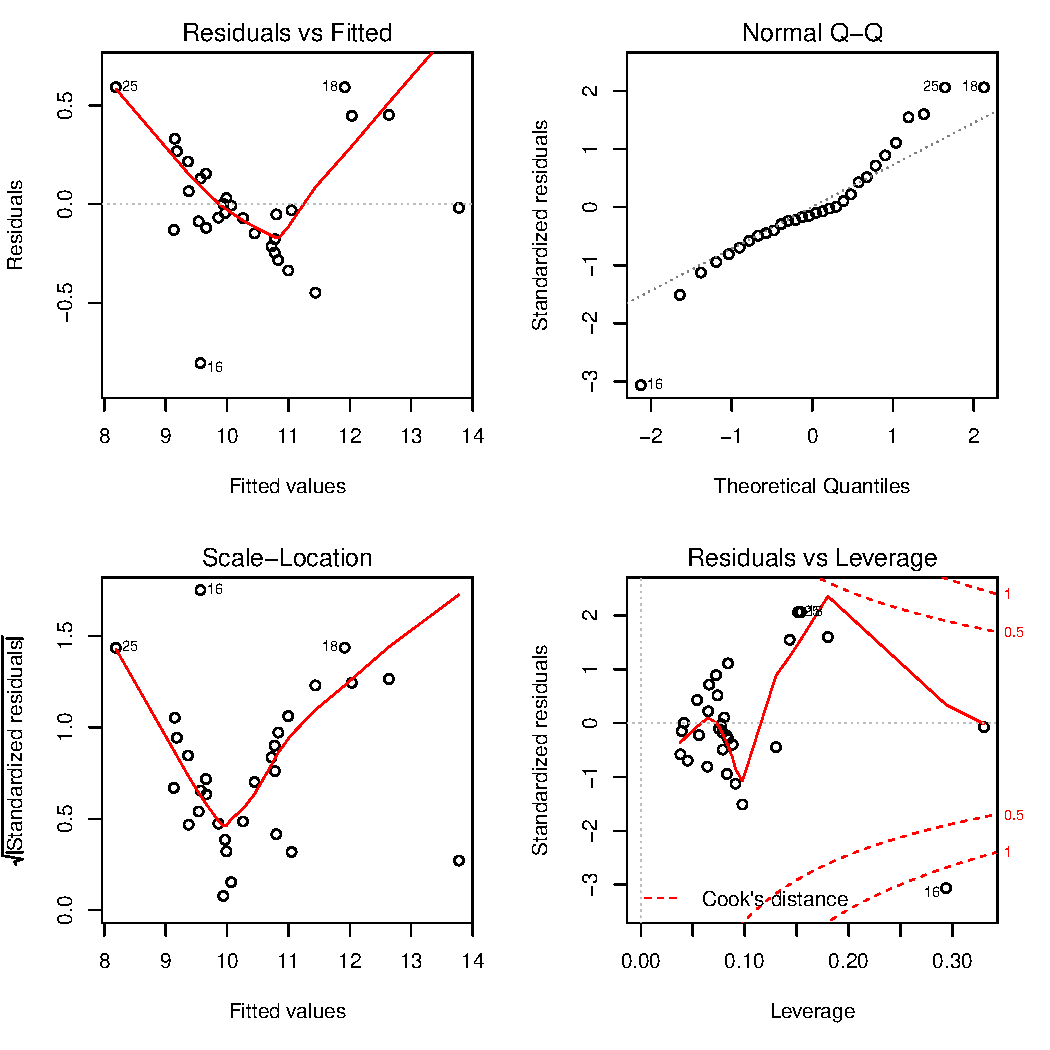
\includegraphics[width=0.8\linewidth]{figure/beamer-unnamed-chunk-27-1} 

}



\end{knitrout}
\end{frame}

\begin{frame}[fragile]{}
Alternatively, we could have mapped the variable {\tt cyl} to the visual property of \rp{shape}
\begin{knitrout}\footnotesize
\definecolor{shadecolor}{rgb}{0.969, 0.969, 0.969}\color{fgcolor}\begin{kframe}
\begin{alltt}
\hlstd{g} \hlopt{+} \hlkwd{geom_point}\hlstd{(}\hlkwd{aes}\hlstd{(}\hlkwc{shape}\hlstd{=}\hlkwd{factor}\hlstd{(cyl)))}
\end{alltt}
\end{kframe}

{\centering 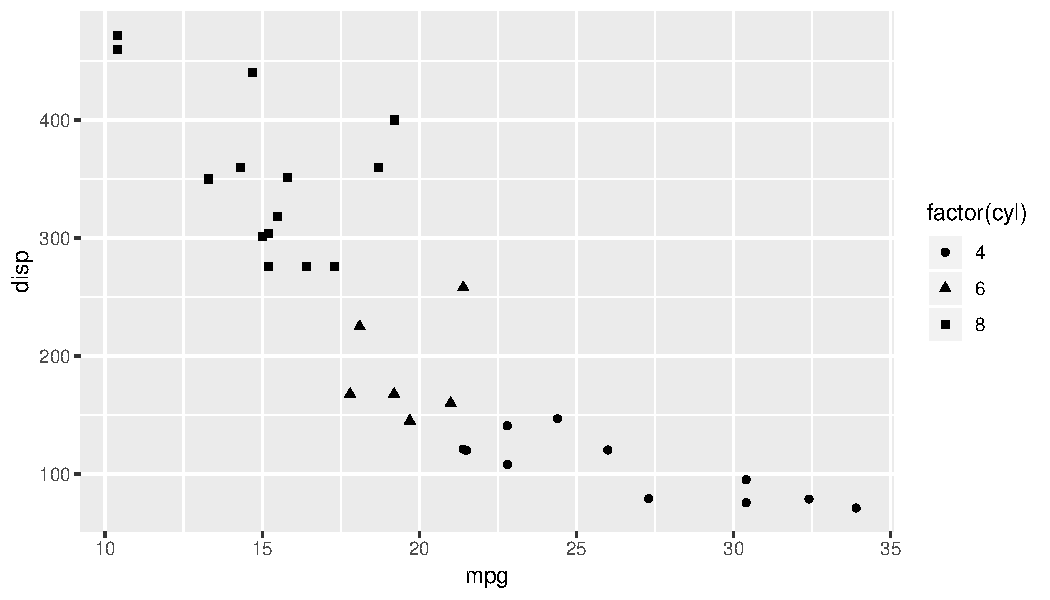
\includegraphics[width=0.8\linewidth]{figure/beamer-unnamed-chunk-28-1} 

}



\end{knitrout}
\end{frame}


\begin{frame}[fragile]{}
Change the transparency and size of points
\begin{knitrout}\footnotesize
\definecolor{shadecolor}{rgb}{0.969, 0.969, 0.969}\color{fgcolor}\begin{kframe}
\begin{alltt}
\hlstd{g} \hlopt{+} \hlkwd{geom_point}\hlstd{(}\hlkwd{aes}\hlstd{(}\hlkwc{color}\hlstd{=}\hlkwd{factor}\hlstd{(cyl)),} \hlkwc{alpha}\hlstd{=}\hlnum{0.4}\hlstd{,} \hlkwc{size}\hlstd{=}\hlnum{5}\hlstd{)}
\end{alltt}
\end{kframe}

{\centering 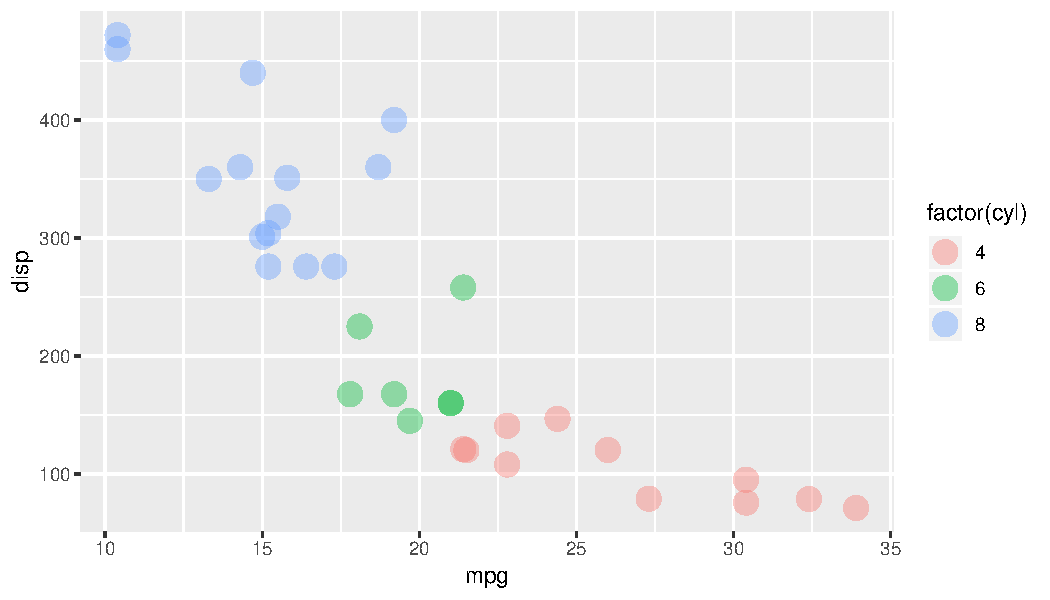
\includegraphics[width=0.8\linewidth]{figure/beamer-unnamed-chunk-29-1} 

}



\end{knitrout}
\end{frame}





\begin{frame}[fragile]{}
Add labels (see slide \ref{auto} for an alternative method)
\begin{knitrout}\footnotesize
\definecolor{shadecolor}{rgb}{0.969, 0.969, 0.969}\color{fgcolor}\begin{kframe}
\begin{alltt}
\hlstd{p} \hlkwb{=} \hlstd{g} \hlopt{+} \hlkwd{geom_point}\hlstd{(}\hlkwd{aes}\hlstd{(}\hlkwc{color}\hlstd{=}\hlkwd{factor}\hlstd{(cyl)))}
\hlstd{p} \hlopt{+} \hlkwd{labs}\hlstd{(}\hlkwc{title}\hlstd{=}\hlstr{"Old cars"}\hlstd{,} \hlkwc{x}\hlstd{=}\hlstr{"Miles per Gallon"}\hlstd{,} \hlkwc{y} \hlstd{=}\hlstr{"Displacement"}\hlstd{)}
\end{alltt}
\end{kframe}

{\centering 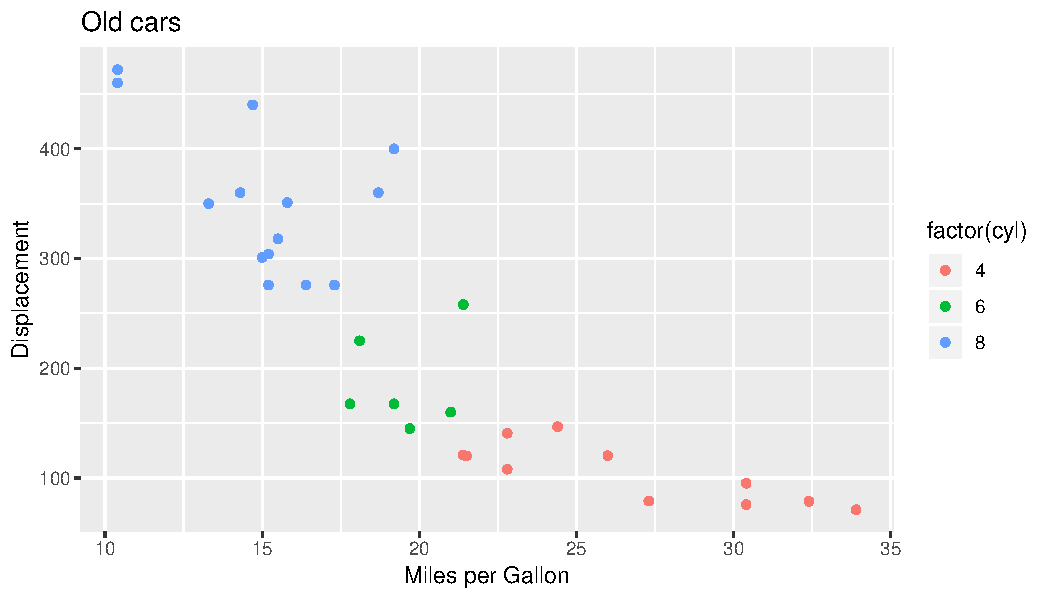
\includegraphics[width=0.8\linewidth]{figure/beamer-unnamed-chunk-30-1} 

}



\end{knitrout}
Notice how labels were added on a separate line of code.
\end{frame}



\begin{frame}[fragile]{Graphs for Qualitative Data: Bar Charts}
\emph{Bar charts} have each group along the $x$-axis and a vertical bar with the height representing the number of observations of each group.
\vfill
See the next slide for an example using the dataset {\tt Auto} in the from the ISLR package:
\begin{itemize}
\item A data frame with 392 observations on the following 9 variables.
\item Gas mileage, horsepower, and other information (9 variables) for 392 vehicles.
\item \ro{orgin} =  Origin of car (1. American, 2. European, 3. Japanese)
\end{itemize}
% \begin{itemize}
% \item A data frame with 392 observations on the following 9 variables.
% \item Gas mileage, horsepower, and other information for 392 vehicles.
% \item Origin of car (1. American, 2. European, 3. Japanese)
% \end{itemze}
% \begin{Verbatim}[xleftmargin=2em, xrightmargin=1.5em, frame=single, numbers=left, label=Frequency Table, framesep=0.5em]
% ggplot(Auto, aes(x=origin))
% + geom_bar(aes(fill=factor(origin)))
% + xlab("") + ylab("") + ggtitle("BARCHART")
% \end{Verbatim}
\end{frame}

\begin{frame}[fragile]\label{auto}
\begin{knitrout}\footnotesize
\definecolor{shadecolor}{rgb}{0.969, 0.969, 0.969}\color{fgcolor}\begin{kframe}
\begin{alltt}
\hlkwd{library}\hlstd{(}\hlstr{"ISLR"}\hlstd{)}
\hlkwd{ggplot}\hlstd{(Auto,} \hlkwd{aes}\hlstd{(}\hlkwc{x}\hlstd{=origin))} \hlopt{+} \hlkwd{geom_bar}\hlstd{(}\hlkwd{aes}\hlstd{(}\hlkwc{fill}\hlstd{=}\hlkwd{factor}\hlstd{(origin)))} \hlopt{+}
  \hlkwd{xlab}\hlstd{(}\hlstr{""}\hlstd{)} \hlopt{+} \hlkwd{ylab}\hlstd{(}\hlstr{""}\hlstd{)} \hlopt{+} \hlkwd{ggtitle}\hlstd{(}\hlstr{"BARCHART"}\hlstd{)}
\end{alltt}
\end{kframe}

{\centering 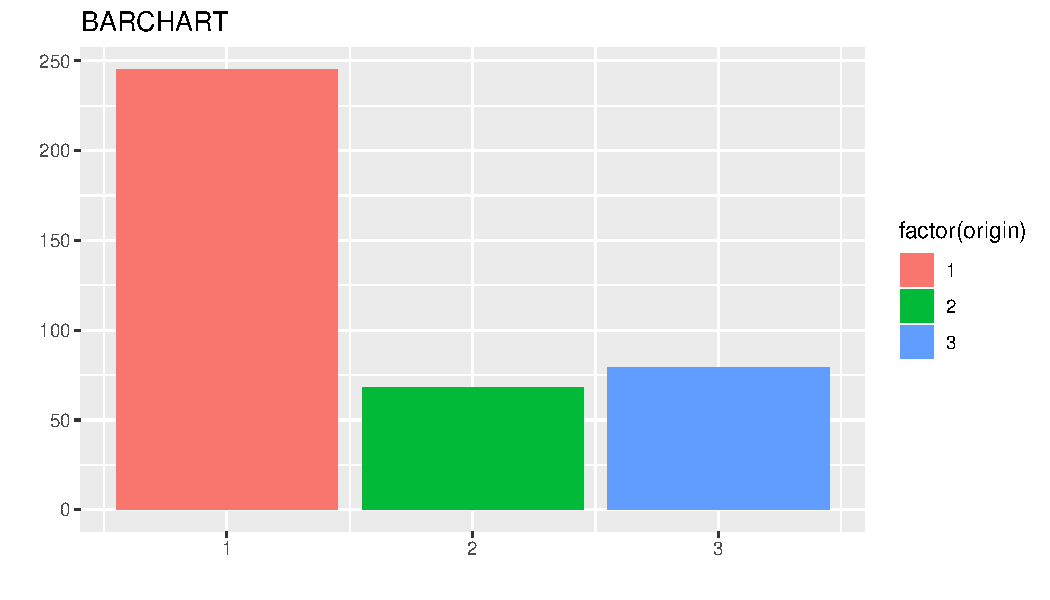
\includegraphics[width=\maxwidth]{figure/beamer-unnamed-chunk-31-1} 

}



\end{knitrout}
% https://ggplot2.tidyverse.org/reference/coord_polar.html


\end{frame}



\begin{frame}[fragile]{Graphs for Quantitative Data: Histogram}

A \emph{histogram} is similar to a bar chart, but the $x$-axis is divided into bins.
\vfill
The variable of interest is on the $x$-axis and the $y$-axis represents count of observations within each bin.
\vfill
Histograms provide a visualization of the data distribution.
\begin{knitrout}\footnotesize
\definecolor{shadecolor}{rgb}{0.969, 0.969, 0.969}\color{fgcolor}\begin{kframe}
\begin{alltt}
\hlkwd{ggplot}\hlstd{(Auto,} \hlkwd{aes}\hlstd{(}\hlkwc{x}\hlstd{=horsepower))} \hlopt{+}
  \hlkwd{geom_histogram}\hlstd{(}\hlkwc{color}\hlstd{=}\hlstr{'mediumvioletred'}\hlstd{,} \hlkwc{bins}\hlstd{=}\hlnum{30}\hlstd{,}
                 \hlkwc{fill}\hlstd{=}\hlstr{'mediumaquamarine'}\hlstd{)} \hlopt{+}
  \hlkwd{xlab}\hlstd{(}\hlstr{""}\hlstd{)} \hlopt{+} \hlkwd{ylab}\hlstd{(}\hlstr{""}\hlstd{)} \hlopt{+} \hlkwd{ggtitle}\hlstd{(}\hlstr{"HISTOGRAM"}\hlstd{)}
\end{alltt}
\end{kframe}
\end{knitrout}
\end{frame}


\begin{frame}[fragile]
\begin{knitrout}\footnotesize
\definecolor{shadecolor}{rgb}{0.969, 0.969, 0.969}\color{fgcolor}

{\centering 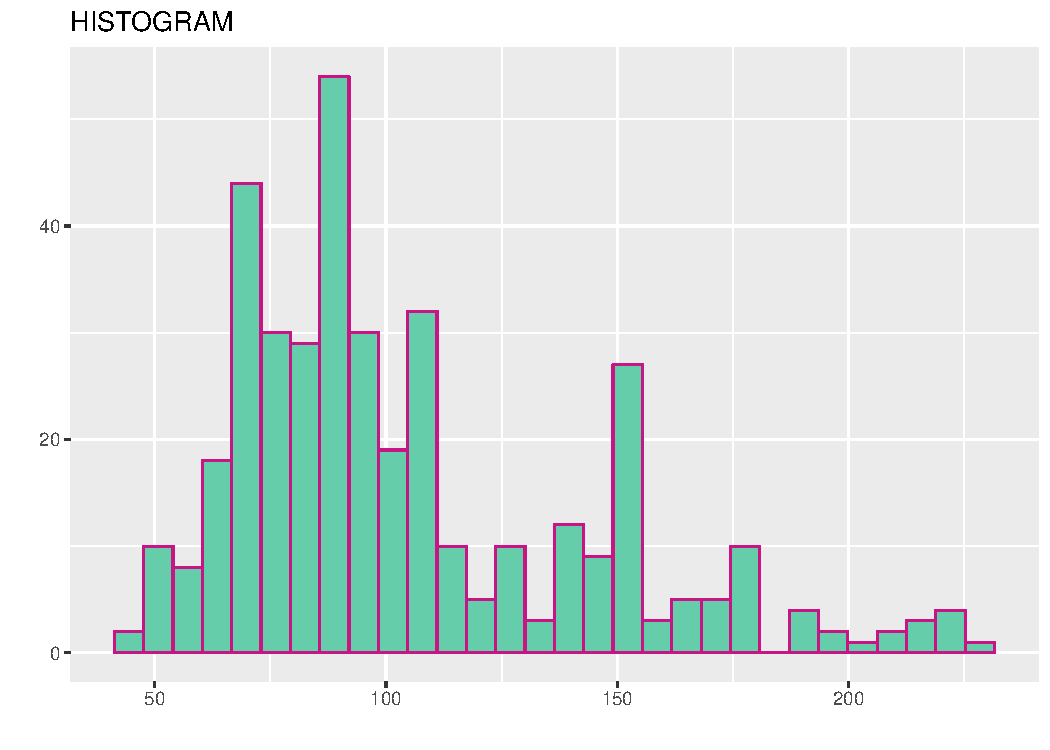
\includegraphics[width=1\linewidth]{figure/beamer-unnamed-chunk-33-1} 

}



\end{knitrout}
\end{frame}



\begin{frame}[fragile]{Graphs for Quantitative Data: Boxplot}
A \emph{boxplot} is a visualization of the five number summary.
\begin{enumerate}
\item Groups along the $x$-axis.

\item Data values along the $y$-axis.
\item Lowest and highest points are the min and max of the data respectively (excluding outliers).
\item Bottom of box is Q1 and top is Q3.
\item Median is represented as the bar inside the box.
\item Single points represent outliers.
\end{enumerate}
\end{frame}


\begin{frame}[fragile]{Boxplot Example Code}
We can create a so-called side by side boxplot by adding the {\tt origin} category as an aesthetic mapping for the groupings along the $x$-axis. 
\begin{knitrout}\footnotesize
\definecolor{shadecolor}{rgb}{0.969, 0.969, 0.969}\color{fgcolor}\begin{kframe}
\begin{alltt}
\hlkwd{ggplot}\hlstd{(Auto,} \hlkwd{aes}\hlstd{(}\hlkwc{x}\hlstd{=}\hlkwd{factor}\hlstd{(origin),} \hlkwc{y}\hlstd{=horsepower))} \hlopt{+}
  \hlkwd{geom_boxplot}\hlstd{(}\hlkwc{color}\hlstd{=}\hlstr{'mediumpurple4'}\hlstd{,} \hlkwc{fill}\hlstd{=}\hlstr{'lavenderblush'}\hlstd{)} \hlopt{+}
  \hlkwd{labs}\hlstd{(}\hlkwc{title} \hlstd{=} \hlstr{"Side-by-side Boxplot"}\hlstd{,} \hlkwc{x}\hlstd{=}\hlstr{"Origin"}\hlstd{)} \hlopt{+}
  \hlkwd{scale_x_discrete}\hlstd{(}\hlkwc{labels}\hlstd{=}\hlkwd{c}\hlstd{(}\hlstr{"American"}\hlstd{,} \hlstr{"European"}\hlstd{,} \hlstr{"Japanese"}\hlstd{))}
\end{alltt}
\end{kframe}
\end{knitrout}
Rather than appearing as {\tt 1, 2}, {\tt 3}, we rename the categoried \verb|"American"|, \verb|"European"|, and \verb|"Japanese"|, respectively.
\end{frame}

\begin{frame}[fragile]{Boxplot Example Code}
\begin{knitrout}\footnotesize
\definecolor{shadecolor}{rgb}{0.969, 0.969, 0.969}\color{fgcolor}

{\centering 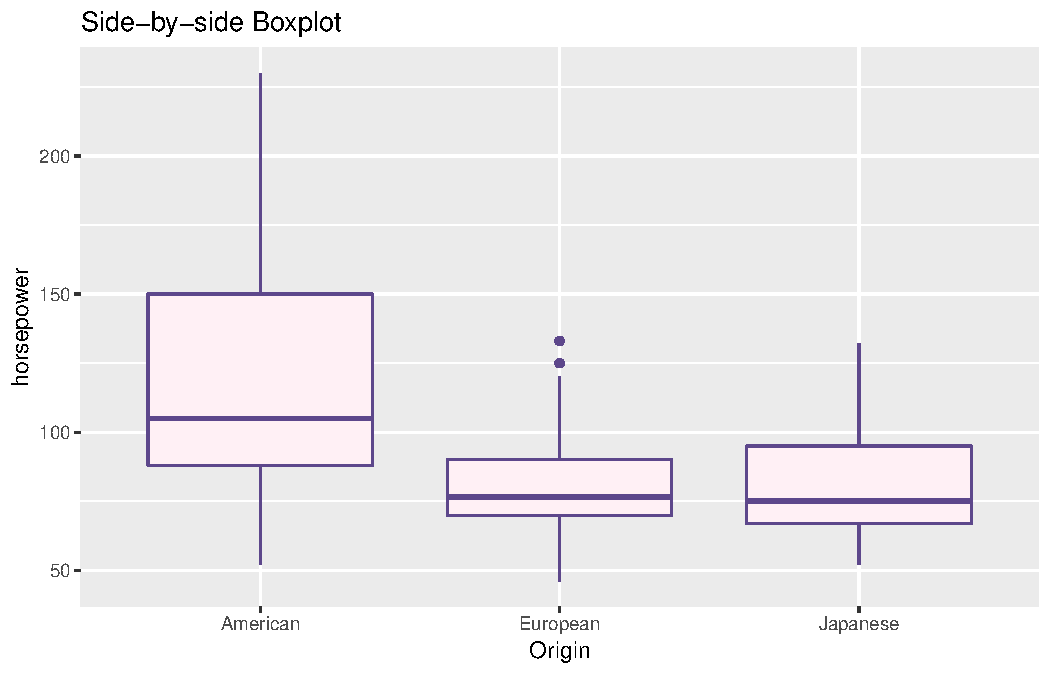
\includegraphics[width=1\linewidth]{figure/beamer-unnamed-chunk-34-1} 

}



\end{knitrout}
\end{frame}


\begin{frame}[fragile]{}
\begin{itemize}
\item Notice how we rename the $x$-axis groupings using \verb|scale_x_discrete| and force {\tt orgin} to a factor using the \rf{factor}\rt{()} function.
\vfill
\item An alternative (and arguably better) method would be to update our data frame prior to doing any plotting:
\end{itemize}
\begin{knitrout}\footnotesize
\definecolor{shadecolor}{rgb}{0.969, 0.969, 0.969}\color{fgcolor}\begin{kframe}
\begin{alltt}
\hlkwd{class}\hlstd{(Auto}\hlopt{$}\hlstd{origin)}
\end{alltt}
\begin{verbatim}
## [1] "numeric"
\end{verbatim}
\begin{alltt}
\hlstd{Auto}\hlopt{$}\hlstd{origin} \hlkwb{=} \hlkwd{factor}\hlstd{(Auto}\hlopt{$}\hlstd{origin,}
          \hlkwc{labels} \hlstd{=} \hlkwd{c}\hlstd{(}\hlstr{"American"}\hlstd{,} \hlstr{"European"}\hlstd{,} \hlstr{"Japanese"}\hlstd{))}
\hlkwd{class}\hlstd{(Auto}\hlopt{$}\hlstd{origin)}
\end{alltt}
\begin{verbatim}
## [1] "factor"
\end{verbatim}
\end{kframe}
\end{knitrout}
\end{frame}


\begin{frame}[fragile]{}
\begin{knitrout}\footnotesize
\definecolor{shadecolor}{rgb}{0.969, 0.969, 0.969}\color{fgcolor}\begin{kframe}
\begin{alltt}
\hlkwd{ggplot}\hlstd{(Auto,} \hlkwd{aes}\hlstd{(}\hlkwc{x}\hlstd{=origin,} \hlkwc{y}\hlstd{=horsepower))} \hlopt{+} \hlkwd{geom_boxplot}\hlstd{()} \hlopt{+}
  \hlkwd{labs}\hlstd{(}\hlkwc{title} \hlstd{=} \hlstr{"Side-by-side Boxplot"}\hlstd{,} \hlkwc{x}\hlstd{=}\hlstr{"Origin"}\hlstd{)}
\end{alltt}
\end{kframe}

{\centering 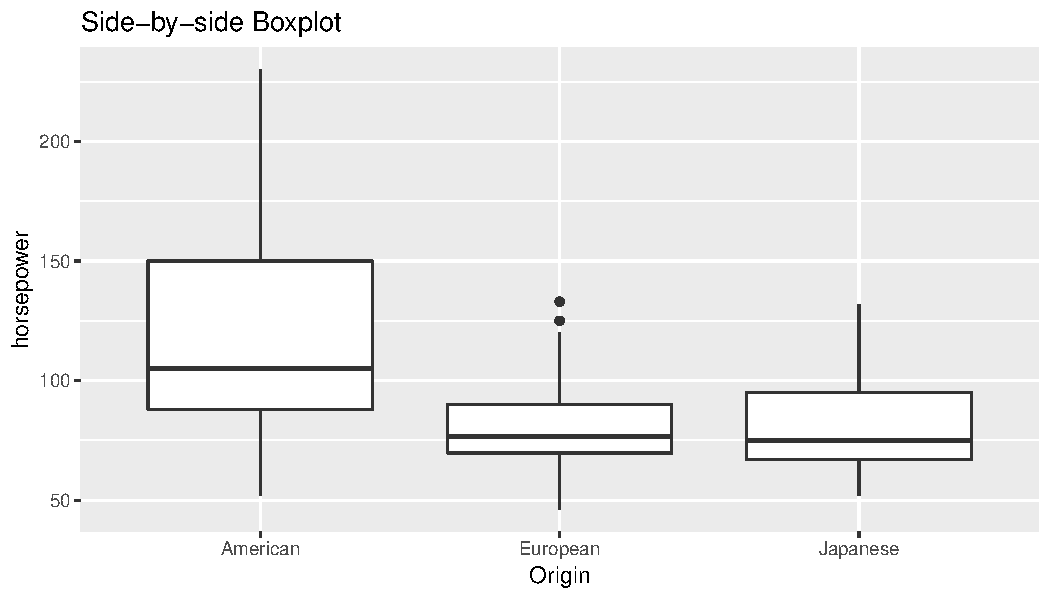
\includegraphics[width=\maxwidth]{figure/beamer-unnamed-chunk-36-1} 

}



\end{knitrout}
\end{frame}

%%%%%%%%%%%%%%%%%%%%%%%%%%%%%%%%%%%
% Question ########################
%%%%%%%%%%%%%%%%%%%%%%%%%%%%%%%%%%%

\begin{frame}[fragile]
\begin{question}
 How many of the are following statements are true?
  \begin{itemize}
\item Colours within the R palette can be referenced by number 
\item Boxplots display the five number summary of a data set. 
 \item The \rf{ggplot}\rt{()} is available in {\bf base} R (i.e. there is no  need to load any packages).  
\item Layers are added to ggplot objects using the {\tt +} operator. 
\end{itemize}
\end{question}
\begin{multicols}{5}
\begin{enumerate}[A)]
\item 0
\item 1
\item 2
\item 3
\item 4
\end{enumerate}
\end{multicols}
\end{frame}


\begin{frame}<handout:0>[fragile]
\begin{question}
 How many of the are following statements are true?
  \begin{itemize}
\item Colours within the R palette can be referenced by number \pcmark
\item Boxplots display the five number summary of a data set. \pcmark
 \item The \rf{ggplot}\rt{()} is available in {\bf base} R (i.e. there is no  need to load any packages). \pxmark
\item Layers are added to ggplot objects using the {\tt +} operator. \pcmark
\end{itemize}
\end{question}
\begin{multicols}{5}
\begin{enumerate}[A)]
\item 0
\item 1
\item 2
\item \tans{4}{3}
\item 4
\end{enumerate}
\end{multicols}
\end{frame}




% \begin{frame}{Summary}
% \begin{itemize}
% \item \ggpp is a very powerful and flexible tool for creating good looking graphics.
% \item While the learning curve may be a little steaper than with {\bf base}, hopefully by seeing plot examples side-by-side, you can appreciate the efficiency of using \ggpp over {\bf base}
% \item This is only a short demonstration of the power of this package.
% \item Explore the difference features using the references provided on slide \ref{refs}.
% \end{itemize}
% \end{frame}



% \begin{frame}[fragile]
% <<eval=TRUE, echo=FALSE>>=
% f <- '08RIII.Rnw'
% knitr::purl(f)
% Stangle(f)
% @
% \end{frame}



\end{document}

